\chapter{家之罪魁}
% 原书第189页

上章提到有关索额图的内容出现在《西征随笔》中“张汧、祖泽深之狱”与“高文恪遗事”两节。这两节的真正目的是回答当时士人普遍关注的两件朝堂上的蹊跷之事。张汧贪污案是康熙朝一件牵涉多位朝廷汉官的案子，由马齐带队彻查。在这个案子中，张汧贿赂徐乾学，高士奇也牵涉其中，这是当时公布过的朝廷政事。但这个案子真正的来龙去脉并不为人所知。特别是徐乾学（1631—1694），他作为顾炎武的外甥，是康熙铲除鳌拜后第一科（1670）的探花，后来成为康熙早年最重要的汉臣之一，官至刑部尚书，声望很高。因而与他相关的贪污案子，当时士人都有兴趣知道。第二件蹊跷之事就是高士奇到底如何以一个秀才身份入值南书房，并进入翰林院。这也是天下士人都深感好奇的。


% 原书第189–190页

《西征随笔》中索额图获罪的关键人物是高士奇。而让两人产生联系的是一个叫祖泽深的人。祖泽深并不是清史中的名人，《清史稿》甚至没有此人的传记。汪景祺在书中一般提到谁，都用当时习惯的称谓，不做相关介绍。但他大概也认为祖泽深不是什么名人，因而多写了几笔：“祖泽深，字仁渊，奉天人，以吏部汉军主事，历官苏松常镇粮道。”主事是六品官，而粮道最多也就是四品。看到这里，随之而来的问题就是：这样的背景凭什么能登上满人权贵之家，还可以给索额图推荐人？而且在汪景祺的故事中，祖泽深还曾经把高士奇介绍给了徐乾学。也就是说，在汪景祺笔下，祖泽深是满、汉两边高层都能说得上话的人。一个四品或者六品的普通官员，很难做到这一点。


% 原书第190页

祖泽深到底是什么人？带着这个问题，查到徐乾学的文集中，有他给祖泽深写的墓志铭。\NoteRef{06}{1}原来，祖泽深是祖大寿的第五子，而祖大寿（1579—1656）是明清之际交战双方互相争夺的一员大将。他在明清两边都曾效力，是明清易代之际的元老武将。努尔哈赤、皇太极、多尔衮、袁崇焕、洪承畴、孔有德等名将都曾和其共过事或者对过阵，他降清后还劝降过吴三桂。所以，作为祖大寿的儿子，祖泽深尽管官阶不高，但却是实打实有大家族背景的人物。祖大寿的儿子能够进入索府以及能与徐乾学往来，符合当时京城的官场秩序。在任何一个政治圈，其实都有祖泽深这样官阶不高，但能量很大的人物存在。


% 原书第191页

《西征随笔》称祖泽深最初发现高士奇，出于两个理由：一是高士奇善于书法；二是祖泽深认为高的面相好，有大前途。在祖泽深把高士奇引荐给索额图后，高士奇便成为康熙书法兴趣的最大受益者。根据官方记载，高士奇在1671年，也就是鳌拜被铲除后两年，因为书法好，得到康熙额外提拔。到底谁给了高士奇机会，让这个举人都没有考上的人能够在康熙面前展示他的字？高士奇的非常经历其实令当时天下悬梁刺股准备科举的人深感不公，以至于在高士奇被提拔了十八年之后，1689年，当高士奇被参劾时，参劾文字的开头还写着“士奇出身微贱，其始徒步来京”，因其“字学颇工，不拘资格，擢补翰林”\NoteRef{06}{2}。高士奇在康熙身边已近二十年，朝廷上下念念不忘的仍然是他的出身。这时的高士奇已享有高官厚禄，但朝臣还是不忘挖苦他“其始徒步来京”。


% 原书第191–192页

根据高士奇自己的记录，他刚到北京时确实是穷困潦倒。他的父亲早年曾在北京做生意，后来因为明清交替时的战乱，回到了浙江。1663年，十九岁的高士奇成了婚。二十岁携妻前往北京，结果第二年父亲去世。高士奇一家在北京的生活陷入拮据，以至于妻子去世后，他在悼亡诗中回忆道，这一时期他的夫人经常去典当发簪和耳环来换取食物；同时，他也提到了这一时期他卖字为生，夫人在旁磨墨的往事。1667年，高士奇曾花钱捐了一个国子监太学生的学籍。一直到1671年，这个学籍才发挥了作用。当时康熙要在国子监中挑选善于写锺繇和王羲之书法的人，高士奇被国子监选为第七名，但康熙亲自测试后，钦定高士奇为第一名，由此改变了他的命运。\NoteRef{06}{3}这一年康熙十七岁，高士奇二十七岁。康熙名义上选的是侍从，为其打理文书，但实际上在后来与康熙的交往中，高士奇渐渐成为了康熙的老师。康熙早年得到朝廷内外认可的明面上的老师是沈荃。他是顺治朝进士，并且是当年的探花，同时又是名满天下的书法家。沈荃也是1671年这一年被指定为康熙的老师。\NoteRef{06}{4}从康熙的回忆来看，沈荃确实如慈父般，一笔一画教他写字。\NoteRef{06}{5}


% 原书第192页

从康熙的学习生涯来看，1671年是康熙真正自主挑选老师，开始深入学习汉文化的年份。那年春，由礼部给康熙选派老师讲课。\NoteRef{06}{6}所以康熙是从十七岁才开始真正系统学习诗、书、礼、易等汉文化课程。尽管还有其他的老师（日讲官）给康熙上课，但康熙与沈荃和高士奇的相处时间最长，因为二人要负责教授康熙书法。对于康熙这个学生来说，沈高二人最大的区别可能就是沈荃1671年时已经四十八岁，而高士奇只有二十七岁，跟十七岁的康熙年龄更接近。这两位老师对康熙的学习可能起到了相似的作用。沈荃1684年去世，康熙给他的谥号是“文恪”。1705年，在高士奇去世两年后，康熙御赐给高士奇的谥号也是“文恪”。前后相隔二十一年。


% 原书第193页

高士奇被康熙选中，获得非同一般的信任，无论当时人还是后来写史的人都认为是经高层特殊安排的结果。《清史稿》说他最早是明珠推荐的，而《西征随笔》说是索额图提拔的。两种说法虽然不同，但都说出了一个简单的道理，就是高士奇背后有人。


% 原书第193–194页

从现存高士奇自己留下的记录来看，他似乎有意避免提及朝中政事，除了记录过与纳兰性德诗文上的交往之外，他没有提过与索额图、明珠或者其他满人权贵有往来。他写下的都是与汉人士子的各种诗文之交。学者武佩圣从书画史角度，认为《西征随笔》中所言高士奇与索额图有关系是一个符合当时情况的说法。\NoteRef{06}{7}因为已知索额图的众多藏品中不仅没有赝品，而且件件皆精，显然背后有高水平鉴定专家在帮他把关。想在高仿遍地，又没有仪器辅助的明清时期，买到的都是真品，其实是很难办到的事。武佩圣强调古画的真伪鉴定是高度专业的技术，每一个大藏家背后的书画鉴定人是谁，在行业中都是公开的。比如索额图以外，当时北京还有另一位大藏家耿昭忠，他是耿仲明的孙子，也是三藩之乱中靖南王耿精忠的弟弟。耿昭忠一直在北京当驸马（额驸），并未受牵连。他鉴定的“手眼”是一个叫陈定的人。\NoteRef{06}{8}而高士奇可以说是当时北京最有水平的书画鉴定家。他自己也说，在1689年回乡后，很多人来找他鉴定，还有很多人拿着画来卖给他。\NoteRef{06}{9}所以武佩圣从书画角度证明《西征随笔》所言高士奇与索额图的关系是有根据的。


% 原书第194页

索额图是索尼的第三子，而索尼家是满人家族中最崇尚文化的家族：索尼的父亲、兄弟都是精通汉、满、蒙三语的人。索额图也不例外，他在1669年就被封为内国史院大学士。\NoteRef{06}{10}但由于索额图后来下狱，他的名字在汉族文人的笔记中很难见到。有记载的大多是在索额图出事前就已去世的文人，比如明末清初著名的小说戏曲家李渔（1611—1680）。他到了京城，受到索额图热情接待，而且就住在索府上。\NoteRef{06}{11}李渔不参加科举，仅靠写作卖书而名满天下，他入京并没有求官与求功名的意愿，所以他与索额图的交往就是建立在文化之上。1673年，他到北京游玩，与故旧相聚，留下许多他与北京各方文人的交往记录。李渔在词中这样赞美索额图：


% 原书第194页

\begin{bookquote}今日朝端，问谁是、斯文宗主。三台上、巍然独建，中原旗鼓。\NoteRef{06}{12}\end{bookquote}

% 原书第194–195页

这是《满江红·呈索愚庵相国二首》第一首的开头。李渔夸赞索额图的角度值得重视：朝堂上崇文，重视中原文化，这是索额图的功劳。“巍然独建，中原旗鼓”这八字说明当时人认可是索额图在推动清廷汉化。这在当时是了不起的功业。1669年，康熙推翻鳌拜。鳌拜代表的正是独崇满洲，与传统汉文化划清界限的国策。满人入关后，一直对汉化抱有很高的警惕性，并采取了一系列措施，包括要把八旗子弟居住地与汉人分开，让八旗子弟享有各种特权，从而确保他们明白自己的出身。就是派到地方的八旗驻军，往往也是专门划定区域居住，不会和汉人混居。\NoteRef{06}{13}所以当鳌拜势力被推翻后，大力提倡在朝廷中引入汉文化，也就是所谓的“建中原旗鼓”，在当时来看是国策级别的转变。当时汉人士子尊称索额图为“索相国”。尽管明朝废除丞相后，中国就没有丞相了，但索额图在当时人心中，拥有丞相的地位。


% 原书第195页

尽管现有的官方历史记录呈现出来的图景是康熙皇帝高瞻远瞩、乾纲独断地推动了清初满人权贵对汉文化的吸收和接纳，但从现实的角度分析，铲除鳌拜时，康熙都还没有正式接受过汉文化的教育，因而真正在皇帝身后建议推动接受汉化大局的人或如李渔所言，正是索额图。如此一来，索额图推荐高士奇给康熙，辅助其学习，于公于私都是水到渠成之事。另一方面，1670年前后，明珠尚未得势，还只是一位御史—明珠真正得势始于三藩之乱后期，也就是1670年代末。在1670年代初，是索额图在打理朝政，因而1671年提拔高士奇的幕后推手是索额图而不是明珠，更符合当时朝政的实际情况。


% 原书第195–196页

关于索额图下狱，《西征随笔》说是已经名满天下的高士奇不堪忍受索额图的羞辱，因而联合明珠除掉了他，其中有一个时间点：


% 原书第196页

\begin{bookquote}癸未年，高随驾北上，时高已叛索，而比明珠矣。\end{bookquote}

% 原书第196页

跟几人同时相关的癸未年是1703年。那一年，有名的大事件是康熙南巡。“高随驾北上”表面上看似乎不通，但经过仔细研读高士奇的经历后，可知他在1689年后，大部分时间都以回家赡养母亲为由住在浙江平湖。而1703年，他奉旨从家里出发到江苏的淮安与南巡的康熙汇合。这次汇合后，高士奇一路随驾巡游，然后又跟着康熙一起回京。所以“高随驾北上”是准确的说法。如果高士奇确实跟在康熙身边，那么接下来的问题是高士奇和康熙的关系到底有多亲密？康熙有可能相信他的话，以至于怀疑自己的老臣索额图吗？


\begin{sectionnotes}

% 原书注释：原书第411页
\BookNote{06}{1}{徐乾学，《憺园文集》，卷29，16b—19a。}

% 原书注释：原书第411页
\BookNote{06}{2}{《清史稿》，列传58。}

% 原书注释：原书第411页
\BookNote{06}{3}{高士奇个人历史，参看王树林，《高士奇年谱》。}

% 原书注释：原书第412页
\BookNote{06}{4}{《清史稿》，列传53。}

% 原书注释：原书第412页
\BookNote{06}{5}{陈捷先，《康熙皇帝与书法》，2。}

% 原书注释：原书第412页
\BookNote{06}{6}{《圣祖仁皇帝实录》，卷35。}

% 原书注释：原书第412页
\BookNote{06}{7}{武佩圣，《王翚客京师期间之交往与绘画活动》。}

% 原书注释：原书第412页
\BookNote{06}{8}{武佩圣，《王翚客京师期间之交往与绘画活动》，618。}

% 原书注释：原书第412页
\BookNote{06}{9}{王树林，《高士奇年谱》。}

% 原书注释：原书第412页
\BookNote{06}{10}{《圣祖仁皇帝实录》，卷31。关于索额图家族背景，参见叶高树，《满洲亲贵与清初政治：都英额地方赫舍里家族的个案研究》。}

% 原书注释：原书第412页
\BookNote{06}{11}{李渔，《笠翁一家言全集》，卷3，40a。}

% 原书注释：原书第412页
\BookNote{06}{12}{李渔，《笠翁一家言全集》，卷8，71b。}

% 原书注释：原书第412页
\BookNote{06}{13}{刘小萌，《清代北京旗人社会》。}

\end{sectionnotes}
\section{高士奇与康熙的关系}

% 原书第196–197页

从官方资料来看，1671年高士奇被选中后最早做的事情是为康熙抄写公文。1677年，康熙在设立南书房近侍职位的时候，直接点名要高士奇，说明高士奇这时已深得康熙赏识。后来康熙无论是北征还是南巡，都把高士奇带在身边。在康熙身边做南书房近侍十二年后，也就是1689年，高士奇遭弹劾。弹劾的核心是他作为皇帝近侍，干预了朝政。南书房近侍的职位类似于皇帝的机要秘书，理论上这个职位是为皇帝打理往来公务，但不能参与决策。由于这个职位的人每天都在内廷办公，设立之初就担心任此职的人会影响外朝之事，所以一开始就说过“勿得干预外事”\NoteRef{06}{14}。但在每天的实际操作中，这个职位的人很难做到不和皇帝谈论朝政。康熙为了平息廷议，让高士奇回乡。高士奇定居平湖。五年后，也就是1694年，康熙又把高士奇召回去继续做近侍。又过了四年，在1698年，高士奇写了一篇以忠孝难以两全为主旨的很富有感情的文章上书康熙，希望康熙准许他回乡赡养老母亲。高士奇称他的母亲在北京水土不服，总得病，而回到浙江几年，病自然好了，因而他请求回乡。至于康熙的知遇之恩，高士奇说只有“他生他世”再来追随。\NoteRef{06}{15}康熙恩准了他的请求。从1698年高士奇再次返乡起直到1703年去世，他和康熙保持着密切的联系。康熙南巡，他也去接驾相见。甚至在1702年，康熙给跟在身边多年的人升官时，还想起了高士奇，说跟高士奇差不多时间入朝为官的都升到了“侍郎”，也应该给高士奇升，遂给他了礼部侍郎的职位。\NoteRef{06}{16}但高士奇以赡养老母为名，没有去赴任。


% 原书第197–198页

从职位上看，就是最后颁给高士奇的“侍郎”也不过是一个从二品的官，而他长年担任的南书房近侍更只是六品的官职，官品远没有达到位极人臣的地步。但对于当时天下人来说，高士奇的能量在于他与皇帝近在咫尺，而不是他的官衔。高士奇一生留下了大量的文字，但由于其所在位置的特殊性，基本没有记录任何朝堂之事，保留的主要是他与文人间的交往。但这些诗文往来，其实恰好反映了高士奇在当时的地位。特别是在他做了南书房近侍以后，北京最有名的士大夫都与他交往密切起来。像比高士奇官阶高、学问名气都很大的王士禛就成了高士奇家中的常客，甚至醉倒在高士奇家中；\NoteRef{06}{17}太子的老师，当时以做官清廉闻名、有“豆腐汤”雅号的汤斌，竟然到高士奇家中，一出手就送了北宋大家李公麟的《赤壁图》。\NoteRef{06}{18}李公麟的画即便在宋代也是天价。高士奇就曾提过有卖家把北宋郭熙的《溪山秋霁图》（现藏美国国立亚洲艺术博物馆）送到他家，但要价过高，他买不起。\NoteRef{06}{19}所以汤斌这个礼物的价值已经远远超过了正常的文人互赠。当时所有在北京的汉人高官可以说都与高士奇常相往来。


% 原书第198–199页

高士奇回乡以后，各路文士自然也是往来不绝。特别值得注意的有两位：冒襄（1611—1693）和黄宗羲（1610—1695）。冒襄《影梅庵忆语》中怀念的与董小宛的爱情生活被后世广为传颂，他的散文也尽显明末士人的风雅。冒襄早年就被称为明末四公子之一，到了清朝更成为名满天下的大家。1690年他派儿子送书信给高士奇，当时冒襄虚岁已经八十。\NoteRef{06}{20}而在1693年，一生孤傲、明末已是士林领袖的黄宗羲，在八十三岁高龄时，主动把自己新写好的书寄给了高士奇。\NoteRef{06}{21}各路文人争相结交高士奇当然不排除是因为他在诗文上也有建树，但按世间人情推测，高士奇在皇帝那里的地位才是他在平湖居家时也门庭若市的根本原因。甚至康熙最得意的包衣奴才曹寅，在1690年上任苏州织造时，也要与赋闲在家的高士奇联络交往。\NoteRef{06}{22}


% 原书第199页

与康熙和曹寅的私人关系相似，康熙与高士奇的关系也是在长时间的朝夕相处中建立起来的。高士奇去世前陪康熙回北京待了一个月后，又要离去。康熙与他话别时说：


% 原书第199页

\begin{bookquote}尔非有军功战阵之事，而以文章事主，始终诚恪，梗直谨慎。朕学问实成于尔。今念尔旧劳，故待尔优渥。尔母老，朕不强尔在京，尔须宽心自爱，弗以离朕为念。朕一二年后仍欲南巡，可以相见，或以诗文事召尔来。\NoteRef{06}{23}\end{bookquote}

% 原书第199页

说这话时，康熙万万没有想到两个月后高士奇就死了，当时还惦记着“一二年后”南巡再相见。这段话其实总结了康熙与高士奇关系的基础：康熙认为高士奇是他的好老师，真的教会了他东西。而康熙认为高士奇好，其实与康熙自己的个人喜好有关。康熙说：


% 原书第200页

\begin{bookquote}当日初读书，教我之人止云熟读四书本经而已。及朕密令内侍张性成钞写古文、时文读之，久而又知张性成不及。后得高士奇，始引诗文正路。他常向我言，诗文各有朝代，一看便知。朕甚疑此言。今朕迩年探讨家数，看诗文便能辨白时代，诗文亦自觉少进，皆高士奇之功。\NoteRef{06}{24}\end{bookquote}

% 原书第200页

传统汉文化的教授，一般侧重于讲解四书五经中的义理，但这部分比较枯燥。康熙最喜欢的其实是传统文化中最具艺术美感的部分——诗文。而这部分正好是高士奇所擅长的。康熙感谢高士奇把他引入了“诗文正路”，而且让他学会了通过看文章的写法，辨别出文章大概是什么年代的人所写。高士奇是“断代”方面的顶尖高手。他鉴定书画真假，核心的基本功就是综合书画的笔法，题跋中的遣词造句，纸、墨等各方面的情况来断代。他教康熙给文章断代，其实是相对容易的部分。


% 原书第200–201页

诗文以外，高士奇擅长的书法和绘画也是康熙的个人兴趣所在。这就注定了高士奇成为康熙的良师益友。比如，高士奇在康熙南巡途中与康熙相会后，康熙让人拿出上千张平时练习的书法，让高士奇品鉴分类，以便未来用作赏赐时可以有所区分。\NoteRef{06}{25}回到北京后，康熙又把几年未到北京的高士奇召入内廷，向他展示自己在书法上的最新进展。康熙告诉高士奇，自己正在学写米芾的字。他按《千字文》的顺序，把米芾书帖中相对应的字找出来，一个一个临摹；如果遇到米芾没有写过的字，再根据他对米芾字的理解来创作。既然老师来了，作为学生的康熙当然要请他来品评一番最近的成果。\NoteRef{06}{26}从高士奇记录的与康熙讨论书法的对话中，似乎康熙还有心在书法上精进，期待成为一代名家：


% 原书第201页

\begin{bookquote}谕云：“凡事贵乎有恒，即一技一能，亦必须久而后成其名。朕于作字留心非一日，今觉稍稍有进。”\end{bookquote}

% 原书第201页

\begin{bookquote}府君（高士奇）奏：“皇上聪明天授，于学问又复精勤。臣昔侍讲幄，深知皇上精一纯粹，好学无倦。”\NoteRef{06}{27}\end{bookquote}

% 原书第201页

康熙学习用功，应该不是高士奇表面上的夸赞。南怀仁以及其他后来教过康熙的传教士都说过差不多的话。康熙练习书法肯下苦功，在很多其他史料中可以得到印证。在这次对话几年后，也就是前面章节提到过的1708年，康熙开始有了心悸的问题，这才渐渐停止练习书法。高士奇在世时，正好是康熙书法兴致最浓的时候。高士奇住在文化荟萃的浙江，一直在留意市场上流通的名作，收购的许多珍品都送给了康熙，后来留存在宫里。\NoteRef{06}{28}


% 原书第201–202页

总结起来，明面上康熙与高士奇是君臣关系，但个人情感上二人惺惺相惜，是亦师亦友的关系。而这种关系能够达到很亲近的程度，还与性格相投有关，这在高士奇记录的许多他与康熙之间的对话中都能看出来。上面引用到康熙对高士奇的评价“尔非有军功战阵之事，而以文章事主，始终诚恪”，“诚恪”二字就是康熙对其性格的总结。现在存留的文字中最能显示高士奇对待身边人态度的，大概是集结了他悼念亡妻诗文的《独旦集》。“独旦”取自先秦古诗《葛生》，意为独自等待天明。在这本书的序言中，高士奇提到他的情况与唐代元稹《遣悲怀三首》中的名句“惟将终夜长开眼，报得平生未展眉”描写的情况相类似。高士奇回乡后三年，在1692年夏天，与他相守近三十年的结发夫人傅氏病故。傅氏除了早年打理家务，还曾在高士奇刚被康熙选中，公务正繁剧时，与其一起检查所写文字之正误直至深夜。\NoteRef{06}{29}对高士奇来说，他与傅氏是患难夫妻，这一点和元稹相似。元稹的悼亡诗名垂千古，原因就在于写尽了识于微时，但未能长相厮守的那份遗憾。陈寅恪评价元稹的悼亡诗“夫唯真实，遂造诣独绝”\NoteRef{06}{30}。高士奇在悼亡诗中展现出来的“真”，不仅是明末清初文坛最为推崇的，很可能也是康熙欣赏高士奇才华的地方。比如在《悼亡诗》三十一中高士奇深情回忆了亡妻在弥留之际，正巧庭院中的茉莉花开了，还拿了几朵放在枕边：


% 原书第202页

\begin{bookquote}时光又见柰花开，侧枕回看意可哀。\end{bookquote}

% 原书第203页

\begin{bookquote}花落有时还更发，人今杳渺不重来。\end{bookquote}

% 原书第203页

\begin{bookquote}自注：亡妻弥留前数日茉莉始开，犹手擎数朵置枕畔，叹曰：“此花又开矣。”\NoteRef{06}{31}\end{bookquote}

% 原书第203页

高士奇还写到妻子临终之际，用手抚着他的面颊，捋着他的胡须，叮嘱他自己保重的场景：


% 原书第203页

\begin{bookquote}最惨临危决绝时，几番执手捋吾髭。\end{bookquote}

% 原书第203页

\begin{bookquote}一声珍重还相嘱，谁料今年是别离？\end{bookquote}

% 原书第203页

\begin{bookquote}自注：亡妻临没时，以手拂吾面，捋吾须云：“三十年夫妇，不道今年永别，此后须自为保重。”\NoteRef{06}{32}\end{bookquote}

% 原书第203页

高士奇这一年悲伤过度，伤了身体。从1693年开始，康熙赏赐高士奇各种补药。\NoteRef{06}{33}其中，四月给他的赏赐，还附带了一封书信：


% 原书第203页

\begin{bookquote}朕少年时最不喜参，尔所素知。只因前岁大病后全赖此药复还元气，所以使人到长白山觅得八九寸长、五六两重者十余根上好者数斤。念尔江湖远隔，苦楚频仍，想是未必如当年气相也，故赐南方所无蜜饯人参一饼，上好人参一斤，土木参二斤。尔当宽心自养，不必多虑。\NoteRef{06}{34}\end{bookquote}

% 原书第204页

“念尔江湖远隔，苦楚频仍，想是未必如当年气相也。”康熙对高士奇的关心已经远远超过了一般的君臣关系。高士奇在妻子去世后，写下了百余首悼亡诗，外加数篇悼文，这些很可能康熙都看过，能感受到高士奇的苦楚。而且单从康熙赏赐高士奇的物品上看，也反映了高士奇在他心中的分量。一些西药，只有康熙有，被称为“圣药”。比如当时传教士在南美发现后，带到世界各地治疗痢疾的金鸡纳树皮。1712年曹寅疟疾病重之时，曾经托李煦找康熙讨这个药救命。\NoteRef{06}{35}也就是说，曹寅和李煦这两位康熙倚重的奴才那里都没有。但康熙却在1690年代多次将这个当时很珍贵的特效药送给高士奇，让他备不时之需。\NoteRef{06}{36}康熙对高士奇的照顾并不体现在加官晋爵这些大事之下，反而是在这些点点滴滴之中。


% 原书第204–205页

1703年，当高士奇陪同康熙回京一个月后又要离开时，康熙万万没有想到高士奇两个月后就遽然离世。在高士奇离京的前一天，也就是1703年6月2日（四月十八日）午后，康熙邀高士奇听曲，并与其话别。康熙在见到高士奇后说：“今日只可谈笑，不可说及离情，涕泣使不尽欢。”\NoteRef{06}{37}在内廷乐师演奏之前，康熙亲自用“西洋铁丝琴”给高士奇演奏了一曲佛教的《普庵咒》。接下来，康熙又命乐师演奏不同的曲目，所展示的都是他最近排练出的新曲。在乐师演奏前，康熙对高士奇说：“朕近以琴谱《平沙落雁》勾作琵琶、弦子、虎拍、筝四乐器同弹。”乐师演奏完毕，高士奇则评价：“四乐合成一声，仍作琴音，声甚清越，极其大雅。”二人最后的欢聚如此安排，很明显，康熙是把高士奇当作了知音。\NoteRef{06}{38}高士奇还记录下了康熙赐酒的瞬间：


% 原书第205页

\begin{bookquote}上先进酒一杯，毕。召臣士奇至御前，上手持金杯盘酒赐臣，云：“知尔素不能饮，明日远行，可略饮之。”臣奏云：“天恩高厚，臣纵不能饮，当尽此杯。”一饮而尽，叩首榻前。时感恩深挚，泪堕杯中。上云：“今日止可尽欢，弗动悲戚。内中女优令尔一观。”\NoteRef{06}{39}\end{bookquote}

% 原书第205页

康熙亲自进酒、高士奇泪堕杯中的感动透过其文字都能感受到。而康熙也很贴心，让他不要伤悲，一起看女优演戏。结束后，康熙还意犹未尽，又把高士奇“召近膝前”倾谈良久。他们又说到画。康熙当然知道高士奇也是行家，命人取出西洋人画的他的“贵嫔”，让高士奇感受西洋画的“逼真”感。聚会结束后，康熙命令侍从搀扶高士奇回去，并叮嘱高士奇：


% 原书第205页

\begin{bookquote}见尔今日甚瘦。尔年虽五十九，精力未衰，相见有日。家有老母，宜一路欢喜而去。\NoteRef{06}{40}\end{bookquote}

% 原书第206页

在康熙眼中，高士奇尽管消瘦，但精力仍然充沛，两人总有再相见的那一天。康熙还给高士奇安排了回程的任务，让他将各种御赐之物分送到江南的一些寺庙。


% 原书第206页

6月3日（四月十九日）是高士奇离开的日子。当天早上，他去领取御赐之物，再次和康熙话别。康熙让高士奇不必悲伤，说：“见尔感涕，朕亦难忍。”然后，吩咐皇十三子送高士奇离开。\NoteRef{06}{41}离开后，高士奇又去了太子处与太子话别。高士奇早年教过太子，很长时间他的正式官衔都是詹事府詹事。詹事府是专门负责太子东宫事务的机构，而高士奇就是这个机构的负责人，因而他与太子也有私交。太子与高士奇又说了很久，除了送了许多礼物，还吩咐用自己的马和骡子把高士奇送往通州去乘船南下。\NoteRef{06}{42}


\begin{sectionnotes}

% 原书注释：原书第412页
\BookNote{06}{14}{《圣祖仁皇帝实录》，卷70。}

% 原书注释：原书第412页
\BookNote{06}{15}{《高澹人行述》，电子版页32。}

% 原书注释：原书第412页
\BookNote{06}{16}{《高澹人行述》，电子版页36。}

% 原书注释：原书第412页
\BookNote{06}{17}{王树林，《高士奇年谱》，28。}

% 原书注释：原书第412页
\BookNote{06}{18}{王树林，《高士奇年谱》，63。}

% 原书注释：原书第412页
\BookNote{06}{19}{王树林，《高士奇年谱》，162。}

% 原书注释：原书第412页
\BookNote{06}{20}{王树林，《高士奇年谱》，115。}

% 原书注释：原书第412页
\BookNote{06}{21}{王树林，《高士奇年谱》，165。}

% 原书注释：原书第412页
\BookNote{06}{22}{王树林，《高士奇年谱》，123。}

% 原书注释：原书第412页
\BookNote{06}{23}{《高澹人行述》，电子版页42。}

% 原书注释：原书第412页
\BookNote{06}{24}{《高澹人行述》，电子版页42。}

% 原书注释：原书第412页
\BookNote{06}{25}{王树林，《高士奇年谱》，268。}

% 原书注释：原书第413页
\BookNote{06}{26}{《高澹人行述》，电子版页40。}

% 原书注释：原书第413页
\BookNote{06}{27}{《高澹人行述》，电子版页41。}

% 原书注释：原书第413页
\BookNote{06}{28}{《石渠宝笈》所著录的清宫内府所藏历代书画藏品有许多是高士奇赋闲在家时收购的，不少作品后都有他写的跋。}

% 原书注释：原书第413页
\BookNote{06}{29}{王树林，《高士奇年谱》，16。}

% 原书注释：原书第413页
\BookNote{06}{30}{陈寅恪，《元白诗笺证稿》，110。}

% 原书注释：原书第413页
\BookNote{06}{31}{王树林，《高士奇年谱》，150。}

% 原书注释：原书第413页
\BookNote{06}{32}{王树林，《高士奇年谱》，150。}

% 原书注释：原书第413页
\BookNote{06}{33}{王树林，《高士奇年谱》，159。}

% 原书注释：原书第413页
\BookNote{06}{34}{王树林，《高士奇年谱》，164。}

% 原书注释：原书第413页
\BookNote{06}{35}{《关于江宁织造曹家档案史料》，98—99。}

% 原书注释：原书第413页
\BookNote{06}{36}{《高澹人行述》，电子版页33。}

% 原书注释：原书第413页
\BookNote{06}{37}{王树林，《高士奇年谱》，270。}

% 原书注释：原书第413页
\BookNote{06}{38}{王树林，《高士奇年谱》，270—271。}

% 原书注释：原书第413页
\BookNote{06}{39}{王树林，《高士奇年谱》，271。}

% 原书注释：原书第413页
\BookNote{06}{40}{王树林，《高士奇年谱》，271。}

% 原书注释：原书第413页
\BookNote{06}{41}{王树林，《高士奇年谱》，272。}

% 原书注释：原书第413页
\BookNote{06}{42}{王树林，《高士奇年谱》，273。}

\end{sectionnotes}
\section{高士奇与索额图的最后时光}

% 原书第206页

高士奇6月3日离开北京后不到一个月，康熙在7月1日就宣布索额图的各项罪状，并把他关入宗人府。而索额图案发后一个多月，高士奇便遽然离世，时在8月12日。事件的演进和《西征随笔》记录的事件发展顺序完全吻合。根据《西征随笔》，高士奇陪康熙南巡回京后，举报了索额图，然后匆匆离开了北京，再然后就是索额图案发。


% 原书彩图3插页（无页码）

\begin{figure}[htbp]\centering
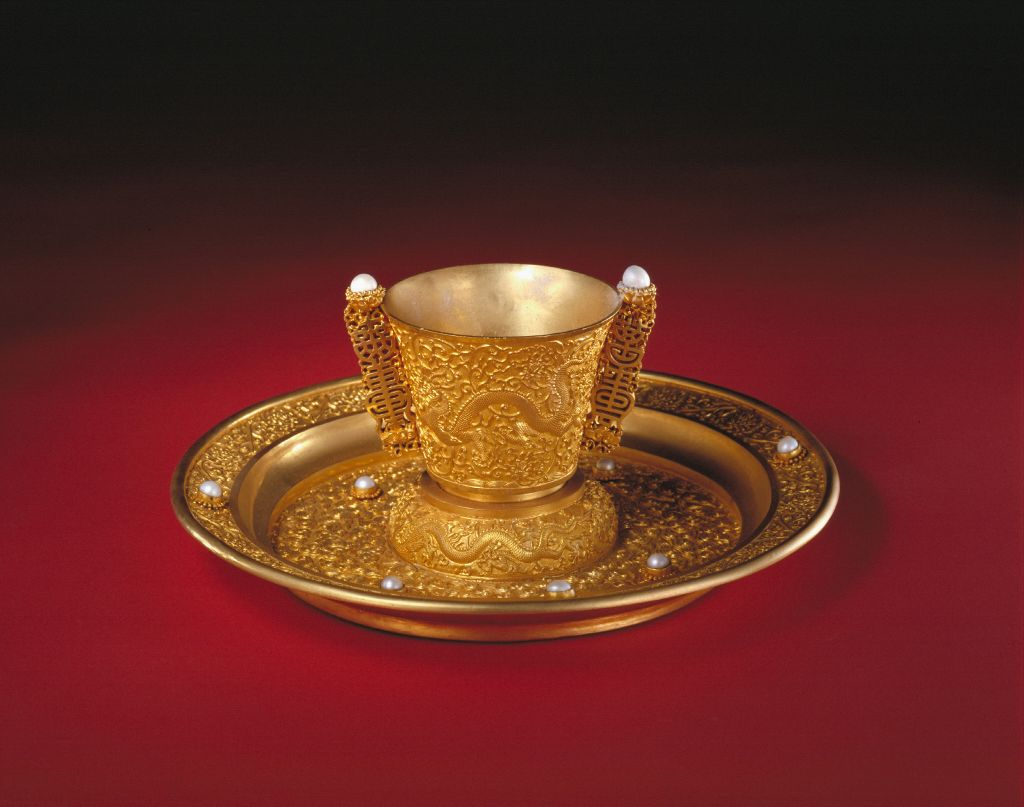
\includegraphics[width=.9\linewidth,height=.68\textheight,keepaspectratio]{assets/cup-dpm.jpg}
\caption{故宫藏清代内务府造金嵌珠“万寿无疆”杯盘（编号：故00012130）}\label{fig:226}\end{figure}


% 原书彩图4插页（无页码）

\begin{figure}[htbp]\centering
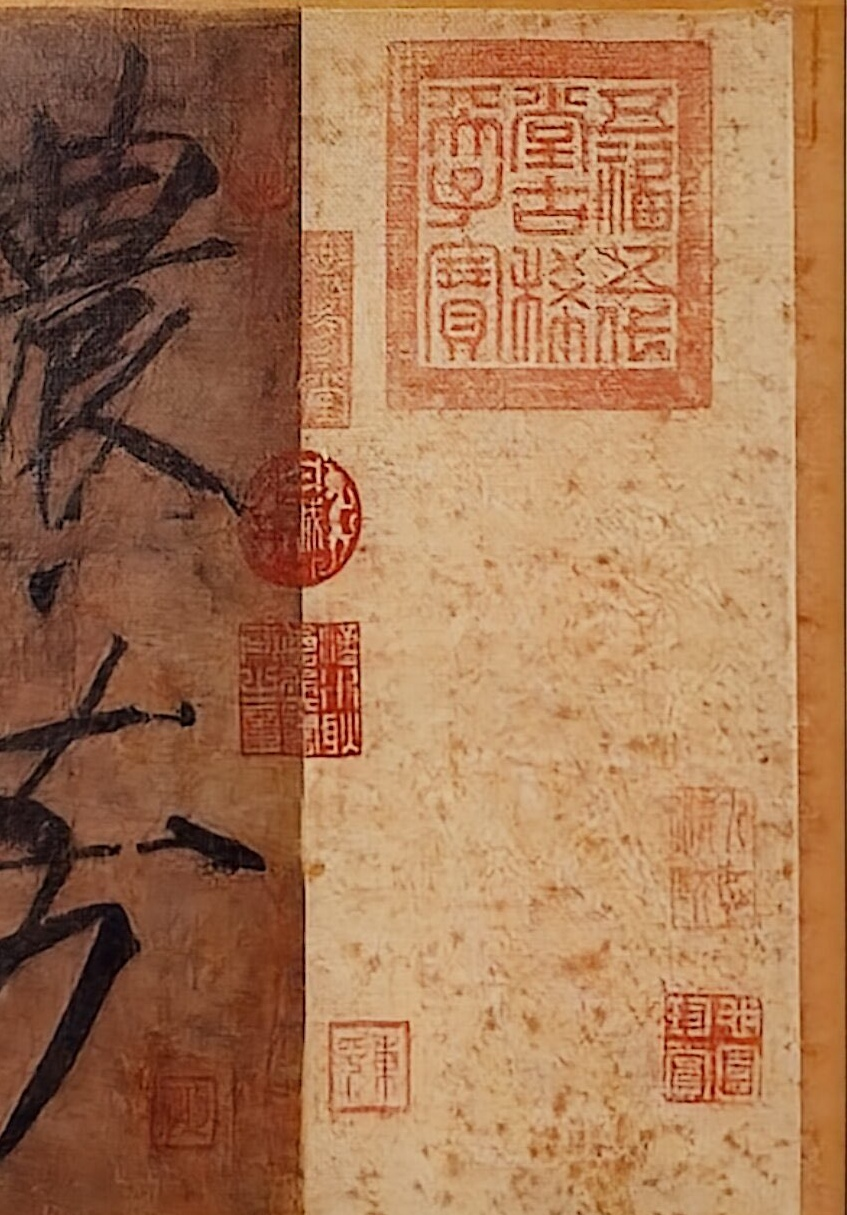
\includegraphics[width=.9\linewidth,height=.68\textheight,keepaspectratio]{assets/fig-227.jpg}
\caption{台北故宫藏《宋赵佶书诗帖》（局部），右下角两方印“九如清玩”“也园珍赏”为索额图印（台北故宫资料典藏检索，编号：中书000001N000000000）}\label{fig:227}\end{figure}


% 原书第207页

另外《西征随笔》中还提到一个让高士奇忍无可忍的人物：江黄。而在《实录》中，康熙曾对索额图说：


% 原书第207页

\begin{bookquote}朕差人搜与尔行走之江潢家，得书字甚多。朕亦欲差人到尔家搜看，但被尔连累之人甚多，举国俱不得安，所以中止。\NoteRef{06}{43}\end{bookquote}

% 原书第207页

也就是说康熙在处理索额图前，确实预先调查过一个叫“江潢”的人。所谓“与尔行走之江潢”，说明这个江潢就是索额图的门客、幕僚一类的人。这和《西征随笔》中提到的那位“江黄”的性质完全一样。“黄”和“潢”固然写法有别，但应该就是同一个人。关于这个历史上不甚知名的人物，《西征随笔》和《实录》两边的记录竟然也对上了。


% 原书第207–208页

《西征随笔》还提示了一个容易忽略的细节，就是当时有传闻高士奇并非正常死亡。汪景祺提到传闻高士奇是被明珠用慢性毒药毒死的。高士奇是6月3日（四月十九日）离开北京，然后去江南各处寺庙为康熙送御赐之物。一直到7月20日（六月七日）才返回浙江平湖的家，然后在8月12日（六月三十日）便去世了。也就是说，高士奇离开北京，以及沿途游历各寺庙时，都还健康，但一到家，很快就去世了。高士奇的儿子高舆记载高士奇去世前一天，在病榻上口授了呈给康熙的遗疏。但这份遗疏高舆并没有公开。后来很多年，高舆还一直有渠道联系康熙。内务府系统的杭州织造孙文成在1706年还在满文奏折中向康熙汇报办理运送高士奇遗物事宜。\NoteRef{06}{44}


% 原书第208–209页

高士奇8月12日（六月三十日）的去世时间和存世的唯一一份索额图的审讯记录似乎也有联系。这份由皇三子与皇八子联署的审讯记录提到他们在1703年8月27日（七月十五日）接到了康熙密旨，于“三更”时分连夜赶去提审关在宗人府里的索额图。从审讯记录中可以看到，索额图自从7月1日被关押以来，管理是比较宽松的。康熙为了照顾索额图，还恩准可以有两个仆人在宗人府里伺候他的起居。而8月27日这次，康熙派两位皇子去调查是谁在帮索额图对外传递讯息。而且很明显事出突然，以至于要连夜调查。审讯记录本身看不出发生了什么事情，但是他俩收到康熙谕旨的时间，是在高士奇去世后十五天，差不多正好是康熙获取了高士奇死讯的时间。最早一封奏报来自驻扎在苏州的江宁巡抚宋荦（1634—1713）。在奏折中，宋荦说他是8月14日（七月二日）收到高舆的书信，得知其父于两天前亡故。宋荦当时正和高士奇一道奉旨校刊一套二十卷的关于诗的书（不知书名），他请康熙下旨做后续的安排。当时为宋荦传递这封奏折的是康熙的包衣奴才苏州织造李煦，他在奏折中也提到了高士奇的死，也就是说康熙最早是通过其包衣奴才的私人通信渠道获知了高士奇的死讯。\NoteRef{06}{45}从宋荦称8月14日接到信息后写了折子并交给同在苏州的李煦，再到李煦写好奏折并派人送往北京，整个过程算下来，差不多康熙就是在8月27日前后收到了消息。而刚与高士奇分别不久的康熙大概率会进一步追查高士奇的死因。所以高士奇的死与索额图被提审很可能有关联。


% 原书第209页

《西征随笔》中提到高士奇非正常死亡的传言，很可能就是出自高士奇的儿子高舆。高舆向世间公布了一份似乎什么都没有说，但又似乎包含许多信息的声明。按照当时的惯例，高舆在父亲去世后写了一份总结其父一生的行述：《皇清诰授光禄大夫礼部侍郎兼翰林院学士加正一品又加二级显考澹人府君行述》。澹人是高士奇的字，很多地方把这篇行述题目中高士奇的官名部分省去，简称为《高澹人行述》。“行述”作为一种为逝者总结一生重要事件的传记性文体，多以正面褒奖为主，但高舆这篇是这样开头的：


% 原书第209页

\begin{bookquote}呜呼痛哉！不孝孤舆何能执笔状我先府君哉？府君遭际圣明，入侍帷幄三十余年，平生忠谟谠论，赞襄密勿者，不语于同列，不告于家人，不孝虽日侍庭除，无从窥测万一。况旻天降割，罹此鞠凶。……\end{bookquote}

% 原书第209–210页

“旻天降割”，语出自《尚书·大诰》中的“天降割于我家”一句。“割”是祸害的意思。高舆说上天降下了祸害，他父亲才“罹此”大凶灾（鞠凶）而去世。高士奇去世时五十九岁，在清代不算早亡。如果高士奇是正常病逝，哪里有儿子会把父亲之死说成天降灾祸的？而且在《行述》中，高舆还把其父临终的病症写得很详细，比如口苦，尿成深黄色，还伴有血迹。而且各方医生来看后，都断定无药可救。这些信息在一般行述中也是不会提及的，似乎高舆意在公布他父亲去世前的细节。


% 原书第210页

另外在高舆称父亲“罹此鞠凶”前，写的是他父亲在朝堂上三十余年不乱讲话，接着便反问为什么会遭此大灾。就算可以接受高舆把父亲去世称为天灾，但他为什么要在行述一开头强调他父亲不乱讲话？正面读这段文字，高舆要说的话是：我父亲一生没有乱讲话，为什么会遭此大难？也就是说他知道他父亲去世跟他父亲说过什么话有关，或者是他知道有人认为他父亲说过什么。在中国传统中，赞美一个逝去的人有各种方式可讲，唯独高舆这里写到的“不语于同列，不告于家人”不是一篇行述展开的正常模式。\NoteRef{06}{46}《西征随笔》提到的高士奇是非正常死亡，和高舆的文字有着某种契合。


% 原书第210页

在高士奇死后来年的新年，康熙委派浙江官员去祭奠，祭词值得重视：


% 原书第210–211页

\begin{bookquote}鞠躬尽瘁，臣子之芳踪；赐恤报勤，国家之盛典。尔高士奇文行优长，才能称职，内廷供奉久劳，方冀遐龄，忽闻长逝，朕用悼焉！特颁祭葬，以慰幽魂。\NoteRef{06}{47}\end{bookquote}

% 原书第211页

表面上高士奇的最后几年是一直赋闲在家，但康熙的“鞠躬尽瘁”四字，暗示他并不是真在赋闲之中。“鞠躬尽瘁”四字本身暗含诸葛亮北伐死于五丈原的典故，并不是一个能随便给出的祭奠之语。而且这四字在康熙心中有着不一般的含义。差不多在第一次废黜太子十年后，康熙在1717年间大病一场，持续了一年。在身体不好，又被群臣催立太子时，康熙向众臣讲了话，后来还告知天下。整个讲话有两千字，反映了康熙晚年的心理状态。\NoteRef{06}{48}他要众臣体谅做皇帝的难，他说“为君者勤劬一生，了无休息”，但做臣子的：


% 原书第211页

\begin{bookquote}臣下可仕则仕，可止则止，年老致政而归，抱子弄孙，尤得攸游自适。\NoteRef{06}{49}\end{bookquote}

% 原书第211页

许多汉人臣子以这样那样的原因请辞，回到家乡，颐养天年。相比之下，做皇帝是一辈子没有休息的职位。在这个背景下，他说出了：


% 原书第211–212页

\begin{bookquote}《易·遁卦》六爻未尝言及人主之事。可见人主原无宴息之地可以退藏。鞠躬尽瘁，诚所谓也。\NoteRef{06}{50}\end{bookquote}

% 原书第212页

《易经》中每个卦有六个爻，代表了该卦六种不同状态。康熙引用《遁卦》六爻，意在说明《易》作为描绘天道规律的书，在遁卦（简单理解为逃遁）的所有状态中都没有讲到“人主”，以此显示皇帝本来就无从休息，也无处可以退藏。他说这就是“鞠躬尽瘁”的意思。而且在这份口谕里，他明确提到了死在北伐中的诸葛亮。康熙完全明白“鞠躬尽瘁”的历史背景，深深知道这个词的含义。所以，他给已经退隐家乡多年的高士奇送上了“鞠躬尽瘁”的祭词，是深思后的赐赠，表明其是死在任务中。


% 原书第212页

而在私下，康熙御书了白居易的一首《山泉煎茶有怀》诗赐给了后来到北京的高舆，表达的是失去知音后的孤寂：


% 原书第212页

\begin{bookquote}坐酌泠泠水，看煎瑟瑟尘。\end{bookquote}

% 原书第212页

\begin{bookquote}无由持一碗，寄与爱茶人。\NoteRef{06}{51}\end{bookquote}

% 原书第212页

至于康熙为何派两位皇子去突审索额图，现有材料尚无法给出定论。但一直到乾隆年间还有士人在记录索额图之倒台与高士奇相关：


% 原书第213页

\begin{bookquote}士奇字澹人，号江村，官至正詹事，谥文恪。癸未索额图之败，根本由此而摇，与有力焉。甲申放回原籍，暴卒，舌本堕地。生时，父梦杨士奇来，因名之，亦由布衣致身通显，盖事非偶然。\NoteRef{06}{52}\end{bookquote}

% 原书第213页

这是乾隆年间萧奭《永宪录》中所记。该书按时间顺序记录了从康熙六十一年到雍正六年间官场中的事。这条关于高士奇和索额图的记录，是因萧奭在写康熙六十一年冬给已经过世的南书房侍从张英追赠头衔时，顺带提到了曾与张英同为南书房侍从的高士奇。而在这样简略的顺带一笔中，就提到了高与索额图之败的关联，可见二者之间的因果在当时官场中也是谈资。癸未年是1703年，所以这一条记录所谓的“索额图之败”就是指其最后下狱那一年的事。而且，萧奭也用“暴卒，舌本堕地”点出了高士奇之死的蹊跷。只是萧奭所记时间上有小错，误以为高士奇是索额图事发后一年（甲申年）才回乡暴毙，实际上距离索额图下狱仅隔了一个多月。萧奭还记录了当时有传言高士奇的名字是效仿明代杨士奇所起，而杨士奇（1366—1444）也是没有科举功名便进入了翰林院，还当了内阁首辅，是明代的奇谈。


% 原书第213–214页

这里需要注意《西征随笔》在民国前并没有在坊间刊刻流传过，因而萧奭《永宪录》是一份独立的史料，并未受到《西征随笔》影响。二者可以互相印证。当然萧奭信笔至索额图，似乎却也不敢多谈他失败的来龙去脉，以及高士奇与他的失败到底有什么关系。从康熙到雍正，无论官方还是民间，在书写索额图相关历史时，似乎都有意要模糊处理。


% 原书第214页

从历史记录这个角度来说，更为不寻常的是清宫档案中现存的高士奇奏折仅有一份（康熙三十九年十月十一日）。这份奏折有三纸，第一纸是向康熙上贡浙江金华的枣子；第二纸讲家中之事，主要是讲他的二儿子生病了；第三纸是写了一首赋。\NoteRef{06}{53}在高舆的《行述》中，可以看到康熙常年给住在平湖家里的高士奇各种赏赐，包括食物、药品、新磨出来的砚台，以及传教士纪理安玻璃厂生产的玻璃制品等等，这表示二人常有联系。\NoteRef{06}{54}上文已经提到过，高士奇的文字只记录与政治不相干的内容，比如康熙送他砚台时一并告诉他是从哪里觅得。这样的事，高士奇才会记录。


% 原书第214页

真正的官场之事，高士奇自己不仅不会记录，他还有可能恳请康熙把通信销毁。太子复立后，康熙让他最为信任的包衣奴才李煦在苏州秘密打探了解江南官场的动向。李煦在上了两次密折后，深感事关重大，在密折中恳请康熙：


% 原书第214页

\begin{bookquote}伏启万岁将臣此折与前次臣煦亲手所书折子同毁不存，以免祸患，则身家保全皆出我万岁之恩赐也。\NoteRef{06}{55}\end{bookquote}

% 原书第215页

李煦当时所查的还只是江南的汉官网络。如果高士奇所查之事是有关索额图或者满人权贵，那不仅是高士奇，就连康熙自己也会步步惊心。这一点并不是无端揣测，从下一节就能看到康熙在让王鸿绪秘密查案时的各种担心。


\begin{sectionnotes}

% 原书注释：原书第413页
\BookNote{06}{43}{《圣祖仁皇帝实录》，卷212。}

% 原书注释：原书第413页
\BookNote{06}{44}{《康熙朝满文朱批奏折全译》，445—446。}

% 原书注释：原书第413页
\BookNote{06}{45}{李煦与宋荦奏折见《康熙朝汉文朱批奏折汇编》，册1，98—99。}

% 原书注释：原书第413页
\BookNote{06}{46}{与高士奇有相同经历、都做过南书房近侍的张英，其子张廷玉也为父亲写过《行述》，同样提到过张英“从无一语及公事”（张廷玉，《澄怀园文存》，卷15，1b）。不乱语公事确实是作为皇帝近侍的一个优点，但高舆所写《行述》的奇怪之处是他把这一点写在了最开头。}

% 原书注释：原书第414页
\BookNote{06}{47}{张诚等纂、王恒修，《平湖县志》，卷首，6b。}

% 原书注释：原书第414页
\BookNote{06}{48}{该谕旨在《实录》中有记录，前人研究中多有提及。最近毛亦可考证发现，在康熙朝刊印的《本朝题驳公案》中对此谕也有记录，因而肯定了康熙确实有过这次真情流露的讲话。参看毛亦可，《康熙末年的“面谕”与第三次立储计划—以〈本朝题驳公案〉新见史料为中心》。}

% 原书注释：原书第414页
\BookNote{06}{49}{李珍编，《本朝题驳公案》，册1，卷5，602。}

% 原书注释：原书第414页
\BookNote{06}{50}{李珍编，《本朝题驳公案》，册1，卷5，602。}

% 原书注释：原书第414页
\BookNote{06}{51}{张诚等纂、王恒修，《平湖县志》，卷首，7a。}

% 原书注释：原书第414页
\BookNote{06}{52}{萧奭，《永宪录》，57。}

% 原书注释：原书第414页
\BookNote{06}{53}{《康熙朝汉文朱批奏折汇编》，册1，48—52。}

% 原书注释：原书第414页
\BookNote{06}{54}{所送物品在《高澹人行述》中多有提及。}

% 原书注释：原书第414页
\BookNote{06}{55}{《康熙朝汉文朱批奏折汇编》，册2，736—737。}

\end{sectionnotes}
\section{王鸿绪查出的密案}

% 原书第215–216页

王鸿绪（1645—1723），江南华亭县人（今属上海），与高士奇有着相似的经历，只不过他是进士出身（1673），高中探花，授翰林院编修，参纂《明史》，后来也入值南书房，比高士奇晚几年出现在康熙身边。他与高士奇私交颇笃，在当时朝中，被认为是高士奇同党。1689年高士奇被参劾时，疏文中就有高士奇“久之羽翼既多，遂自立门户，结王鸿绪为死党”之语。\NoteRef{06}{56}王鸿绪也是当时的书法名家，从其奏折中的小楷便能窥见一二。除了在朝是同僚以外，他们两人还都是书画藏家。据艺术史学者考证，高士奇死后，他的许多书画都被王鸿绪接手。\NoteRef{06}{57}对于康熙来说，高士奇比王鸿绪在私人关系上更亲近一层。但总体上说，二人都属于来自江南的汉人士子；而在后世的历史研究者看来，王鸿绪与高士奇的最大不同在于，王鸿绪有约五十通特殊小尺寸的密折保存了下来，使后世能够一窥当时康熙为其安排的秘密任务。如果说高士奇与王鸿绪在康熙朝扮演着相似的角色，那么或许可以推测高士奇曾经被康熙安排了相似的任务，最后“鞠躬尽瘁”。


% 原书第216页

清宫档案中有一张康熙手写的密谕，要求追查拐骗苏州女子的事：


% 原书第216页

\begin{bookquote}前岁南巡，有许多不肖之人骗苏州女子，朕到家里方知。今年又恐有如此行者。尔细细打听，凡有这等事，亲手蜜蜜（注：秘密）写来奏闻。此事再不可令人知道，有人知道尔即不便矣。（见图片\ref{fig:241a}）。\end{bookquote}

% 原书第216页

这是一份手写的密谕。收件人、时间等基本信息都没有，令人不禁生疑：康熙为何不走朝廷渠道，而要用密谕形式查“骗苏州女子”的案子？他不仅用了密谕交代任务，行文中还要强调“不可令人知道”，甚至还叮嘱收件人“有人知道尔即不便矣”。为什么皇帝吩咐追查一件看似普通的案子，会有这么多的担心?


% 原书第216页

由于这张手写密谕被发现时和王鸿绪的密折放在一起，再加上王鸿绪确有向康熙汇报他查到的苏州女子被骗的密折，所以基本可以确认这张密谕的接收人就是王鸿绪。通过现存他和康熙往来的密折来看，在这次查办苏州女子案前，康熙已经多次交代王鸿绪办案，他都很好地完成了任务。\NoteRef{06}{58}


% 原书第217页

王鸿绪看了康熙密谕中的行文用词，应该知道让他去查的不是普通拐卖案子。在回奏的密折上，他首先表明已经领会了康熙的保密要求，说他收到“密封御批”后，马上就回了家，到家之后才“启封密看”；他还把“亲手密密写来奏闻，不可令人知道”句抄写出来，表示感谢康熙对他的保护，同时也向康熙表明他上的密折从来都是自己亲手书写。


% 原书第217页

王鸿绪查到的案子当然不是一般的拐卖妇女案。他在密折中一开始就列举了好几桩苏州地方官员参与其中的民女买卖。密折中查到的最关键的人物是前东平州的知州—一个叫范溥的人，当时在北京候补了一个官差。此人的麻烦之处在于他“在京各处牵扯”。王鸿绪举了一个例子，说范溥领赏得到过一支“御箭”，而他拿着“御箭带领娼妓行走”。接着王鸿绪报告，范溥买卖的人口还包括男子：


% 原书第217页

\begin{bookquote}范溥在常熟县以银五百两，强买赵朗玉家人之子。其子并非戏子。\NoteRef{06}{59}\end{bookquote}

% 原书第217–218页

根据清代的法律，奴仆等贱民阶层的人可以买卖，但禁止买卖平民，所以王鸿绪特意注明了强买的是“平人子女”。在这个强买过程中，有苏州的地方官在协助。而与北京最有关联之处是这些交易都打着御前人员的名号在进行，“其着落总不可问”。买卖中还有“小手玉蛹”的暗号。“男曰小手，女曰玉蛹”，王鸿绪称他也不知道这是出自什么典故。同时，王鸿绪查到一些案例，表明康熙身边的侍卫以及内务府的官员确实是买家，涉入案中。王鸿绪认为这个案子查起来很困难：


% 原书第218页

\begin{bookquote}此外纷纷买人者甚多，或自买，或买来交结要紧人员。皆是捏造姓名，虚骗成局。\NoteRef{06}{60}\end{bookquote}

% 原书第218页

但最后表示他会继续追查，有了新发现再报告。


% 原书第218页

其实看完王鸿绪的这份密折，就能理解康熙为什么要再三叮嘱王鸿绪秘密查案肯定有蛛丝马迹让康熙知道他身边有人在买卖人口，而且就像王鸿绪所言“纷纷买人者甚多”。王鸿绪接下来的第二份密折，显示他在查案中开始害怕了。


% 原书第218页

第二份密折提到他四月二十四日在扬州见过康熙。奏折一开头便解释，由于康熙在船上这一路，以及刚回北京时他都没找到合适的时机，害怕那时禀奏此事会“露行迹”，所以才拖到现在。王鸿绪在折中先列举了一些他查到的买卖人口的事，然后总结道：


% 原书第218页

\begin{bookquote}扬州商纲到苏买人不一而足，但以上皆彼此明买，并非诓骗。\NoteRef{06}{61}\end{bookquote}

% 原书第219页

写完明买的以后，王鸿绪指出前面提到过的范溥情节比较恶劣，是勾结官府在强买。他再一次提到上回说过的赵朗玉家小童，其母曾到苏州虎丘告官，但被官府压了下去。而那时康熙刚到过虎丘，当地官员士绅还争先前往送驾。范溥没有去，并告诉他的亲戚程某：


% 原书第219页

\begin{bookquote}有汉大臣说我不好，我不去送驾。\NoteRef{06}{62}\end{bookquote}

% 原书第219页

程某也很好奇范溥是怎么能获取到这样的内部信息，问他是否从太监那里得到的。范溥没有直接回答，而是说：


% 原书第219页

\begin{bookquote}不是太监，是御前第一等人与我的信。\NoteRef{06}{63}\end{bookquote}

% 原书第219页

看到这里，康熙在这句话的旁边批注了：


% 原书第219页

\begin{bookquote}此第一等人是谁？（见图片\ref{fig:241b}）\end{bookquote}

% 原书第219页

范溥知道有汉大臣在康熙身边说他不好，而王鸿绪前不久才在折子里对康熙说过范的不是，因此就算不知道范指的是不是自己，他应该都是十分紧张且担忧自己的处境。王鸿绪下面一段话彻底暴露出了他的惊慌：


% 原书第220页

\begin{figure}[htbp]\centering
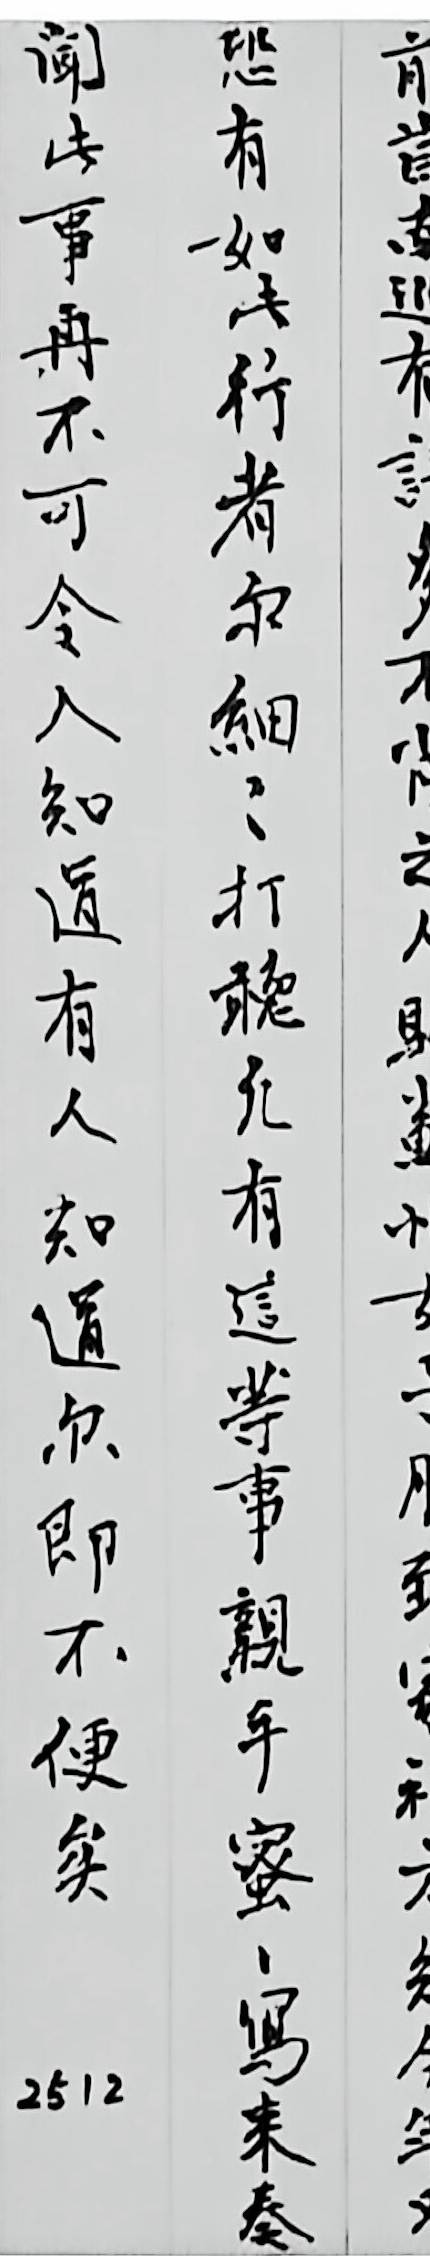
\includegraphics[width=.9\linewidth,height=.68\textheight,keepaspectratio]{assets/fig-241a.jpg}
\caption{康熙密谕王鸿绪奏前岁南巡时有人骗苏州女子事（台北故宫博物院清代档案检索系统，故宫002512号）}\label{fig:241a}\end{figure}
\begin{figure}[htbp]\centering
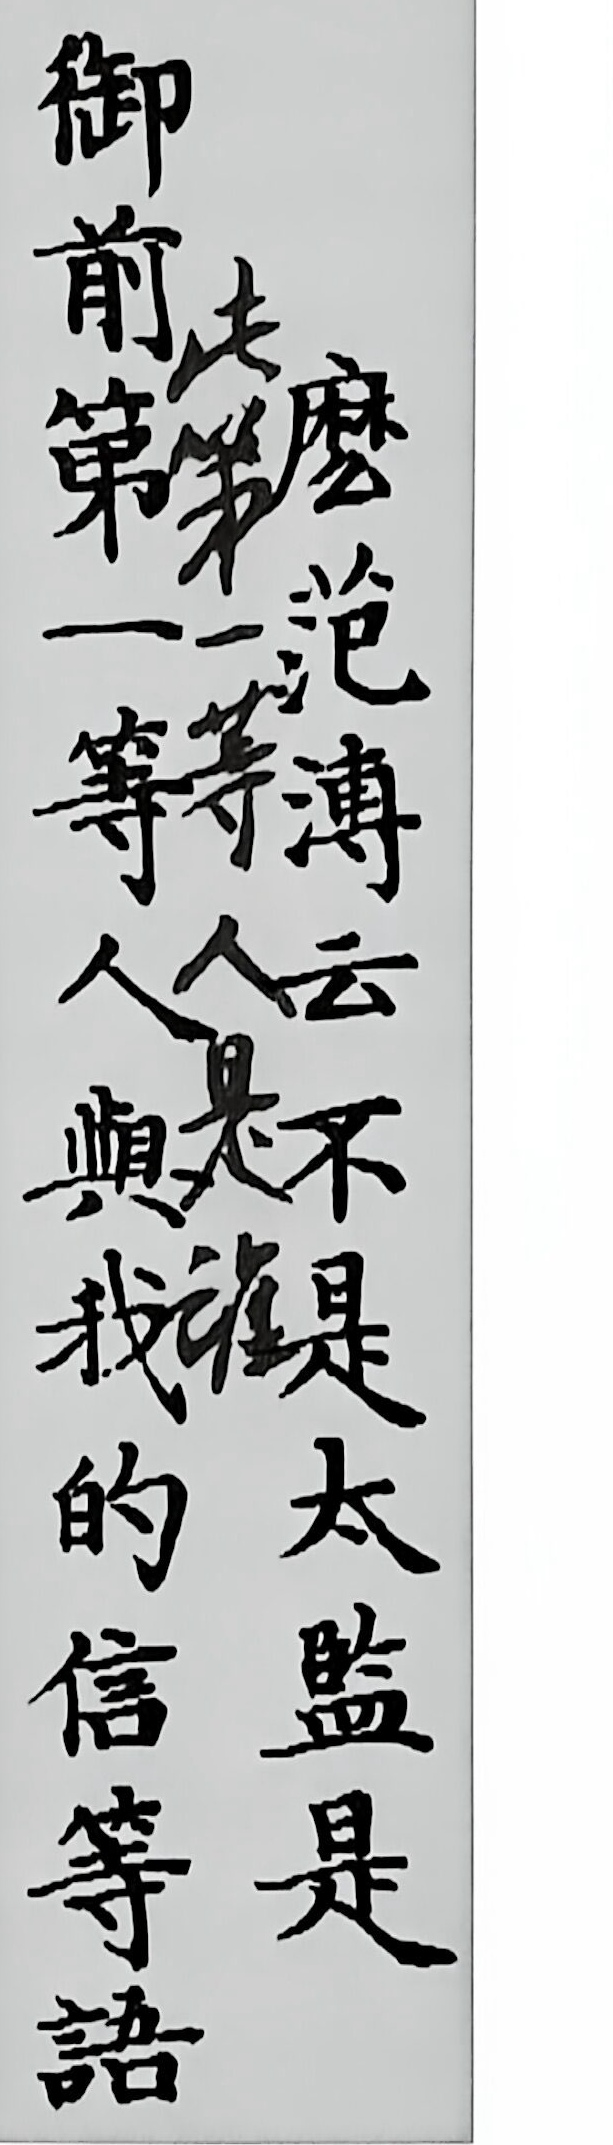
\includegraphics[width=.9\linewidth,height=.68\textheight,keepaspectratio]{assets/fig-241b.jpg}
\caption{工部尚书王鸿绪奏报访得范溥等人纷买苏州女子情形折（部分）及康熙朱批（台北故宫博物院清代档案检索系统，故宫002538号，件1）}\label{fig:241b}\end{figure}


% 原书第221页

\begin{bookquote}范溥在山东包揽捐纳，又系查昇第二子之亲家，平日引其结交侍卫及各王府以下杂色人等甚多，故有人送信与之是真。以范溥之神通广大，加以查昇之多言好事，臣将来必受其中伤。\NoteRef{06}{64}\end{bookquote}

% 原书第221页

这里面提到的查昇（1650—1707）是1688年进士，翰林院编修，入值南书房，供奉内廷。查昇来自浙江海宁查家，属于江南望族之人，王鸿绪对他很忌惮。同时，范溥还结交了满人中的侍卫和各王府中人，这些都是王鸿绪不愿招惹的对象。此外，王鸿绪竟然还直接建议康熙要小心：


% 原书第221页

\begin{bookquote}恐近来时候不同，有从中窥探至尊动静者，伏祈皇上密密提防，万勿轻露，随事体验，自然洞鉴。\NoteRef{06}{65}\end{bookquote}

% 原书第221页

1707年的康熙已经五十四岁了，像这样臣下直接指点康熙该如何行事的密折是很少见的。这也说明王鸿绪在查案过程中已经感觉到这个案子背后所牵扯到的势力很强，而且就在康熙周围。


% 原书第221–222页

在折子的最后，王鸿绪叮嘱康熙一定要让人将谕旨当面交到他的手中，“以免旁人开看”。康熙一反常态，在奏折的最后竟然没有按照习惯批上“知道了”，而是留了一个“是”字，表示他会按王鸿绪所说的做。\NoteRef{06}{66}


% 原书第222页

接下来，王鸿绪继续追查的方向就成了谁是这个所谓的“御前第一等人”。从他再次上的密折看，也许他始终不知道是谁，但也有可能是知道了不敢说，只有抄录出来，留待以后研究：


% 原书第222页

\begin{bookquote}………初得范溥告诉伊戚之语，心中畏惧异常。即托人再访问其所言“第一等人”，还是亲近侍卫们？还是更在上一层的人？程姓云：“这不敢说。”因此不得其人名。臣在扬州时，复托人回苏再访之程姓。昨得家信云“程姓说这人岂是平等，我万万不敢说的”等语。谨先据此密奏。\NoteRef{06}{67}（见图片\ref{fig:244}）\end{bookquote}

% 原书第222页

这封密折后面部分就讲的是苏州当地其他治安事件了，这个案子的追查到这里也就结束了。而康熙在这份奏折的最后用朱笔批注道：


% 原书第222页

\begin{bookquote}范溥一事再无一人知道。若有人说出，非侍卫马五说了。“第一人”（注意：这里用词变成了“第一人”，而非之前的“第一等人”）却一点不知从哪里说起？\NoteRef{06}{68}\end{bookquote}

% 原书第222页

康熙和王鸿绪究竟是真不知道，还是他俩互相装不知道？王鸿绪是真没有查到，还是借用程姓说出“万万不敢说的”几个字？案子查到这里，康熙竟然没有进一步的指令了。如果两人真想知道，把范溥或者那位程姓亲戚抓来一审便知，整个案情马上就会水落石出。但康熙竟然什么都没有做，这完全不符合他雷厉风行的作风。其实什么都不做的原因只可能有一个，就是康熙已经知道或者大概猜出了谁是“第一等人”，但他不想把事情闹大，只能装作不知道。如果提审这两人，他们把“第一等人”以及整个网络牵扯出来，康熙该如何收场？本书第四章就提到过，康熙没有去索额图家搜查，就是怕“连累”太多人，举国不得安宁。康熙作为皇帝不仅要查案，还要思考下一步，查到了又能怎么办？他需要利弊权衡，这不是简单的是非问题。\NoteRef{06}{69}

% 原书第223页

\begin{figure}[htbp]\centering
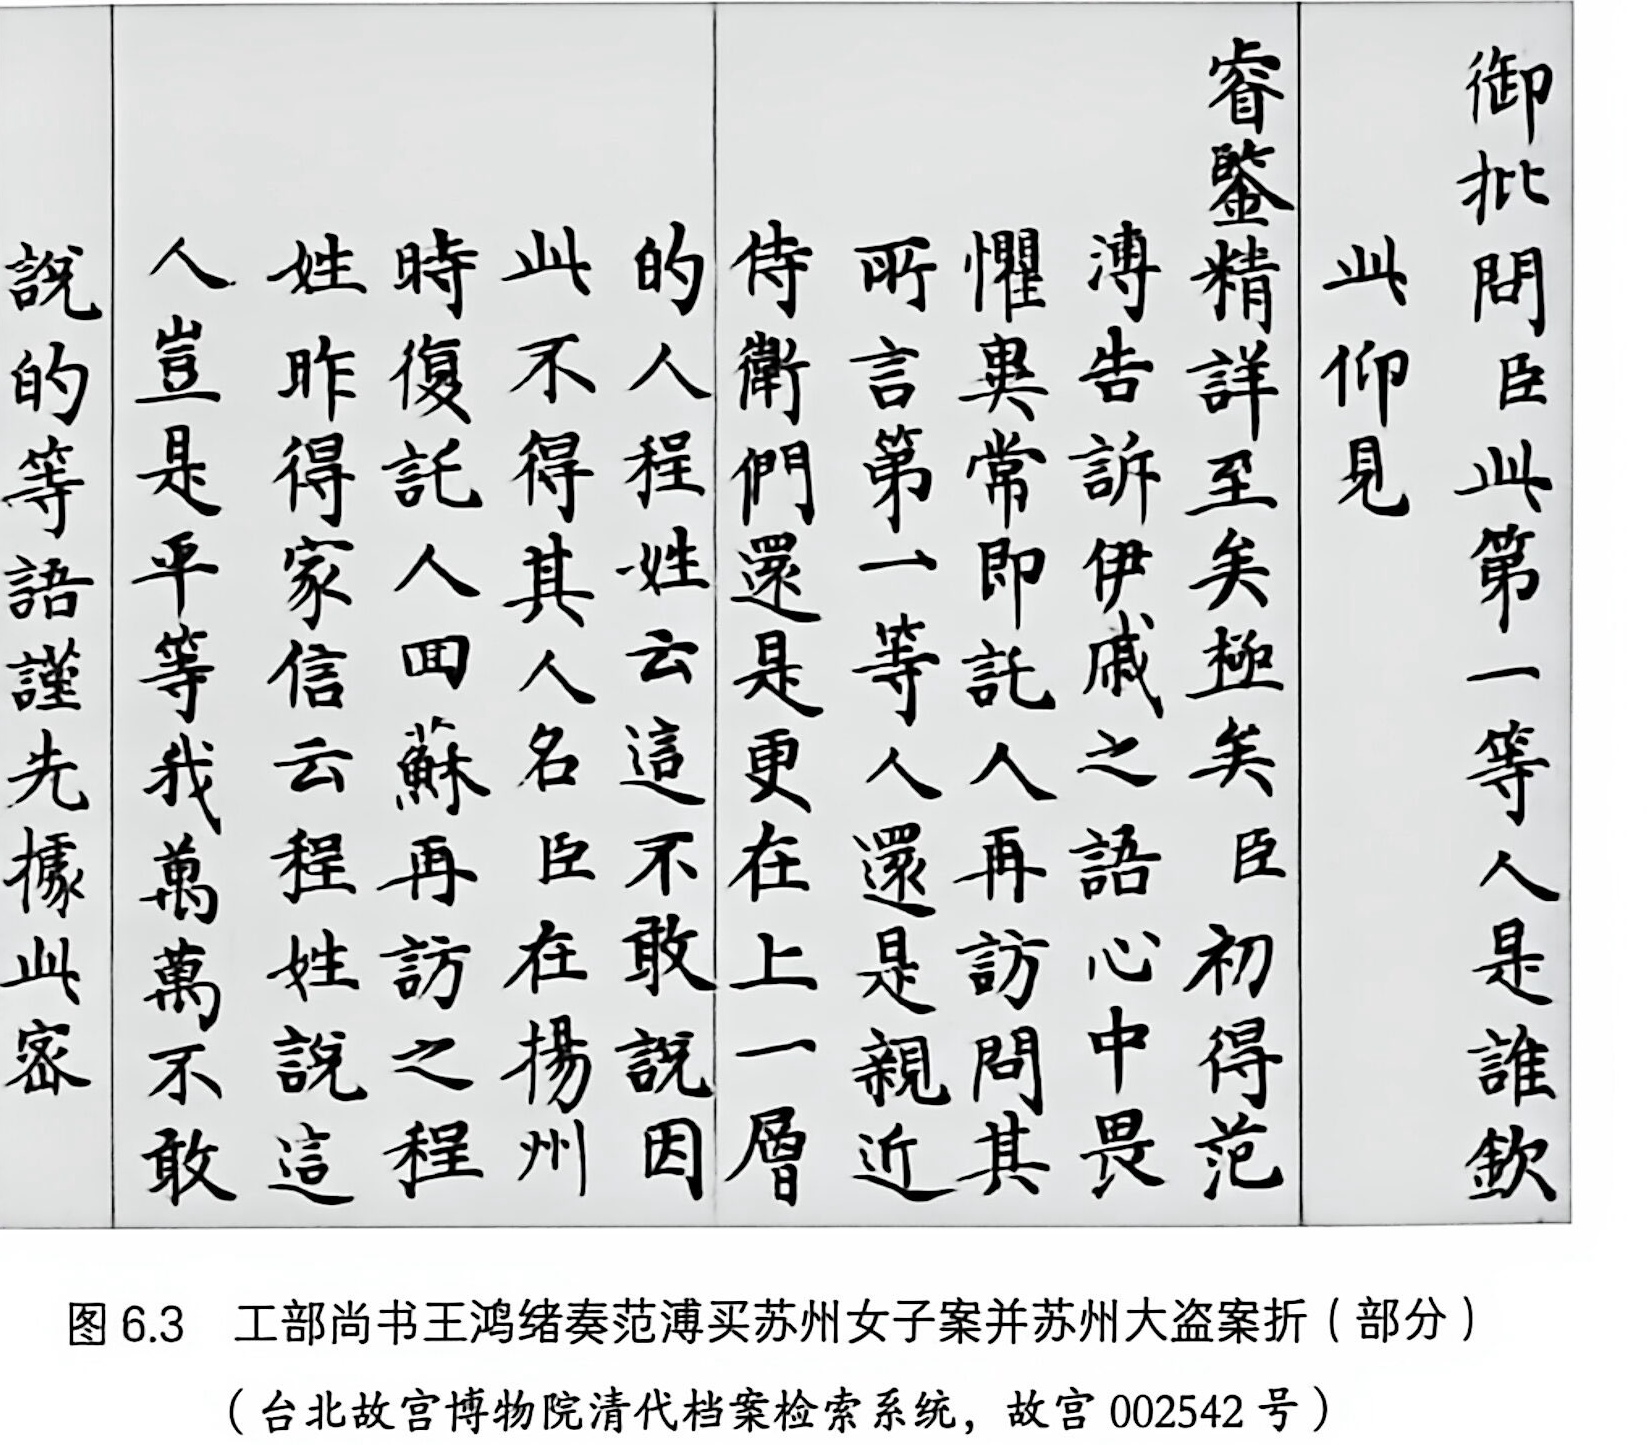
\includegraphics[width=.9\linewidth,height=.68\textheight,keepaspectratio]{assets/fig-244.jpg}
\caption{工部尚书王鸿绪奏范溥买苏州女子案并苏州大盗案折（部分）（台北故宫博物院清代档案检索系统，故宫002542号）}\label{fig:244}\end{figure}


% 原书第224页

根据现有奏折可知，这个苏州买人的案子应该就这样算了，没有继续追究。因为主犯范溥毫发未伤，后来还出现在两年后李煦写的一封与此案完全没有关联的奏折里。而且李煦大概也不知道康熙识得此人，还专门向康熙介绍说是“东平州知州”，“熟于京师要路”。\NoteRef{06}{70}所以康熙和王鸿绪很大可能都知道了“第一等人”是谁，只是“第一等”到了无法追究的地步。


% 原书第224页

两位已故的康熙研究专家吴秀良和史景迁都认为“第一等人”指的就是“太子”。\NoteRef{06}{71}太子确实是最合理的解释。涉及的每一个人，都不愿意也不敢提，甚至康熙自己也不愿意追查，因为追查下去反而会让他这个父亲陷于尴尬的境地。对于康熙来说，要知道是谁并不难。这个案子涉及1705年和1707年两次南巡。前一次随行的只有太子和皇十三子。\NoteRef{06}{72}后一次随行的包括：太子、大皇子、皇十三子、皇十五子和皇十六子。两次都在的人是太子和皇十三子。康熙只要稍微整理一下思路，就知道是谁才能让各方面都“万万不敢说的”。


% 原书第224–225页

还有一点值得注意，就是查过案的王鸿绪在不久之后废立太子时期的表现，完全背离了汉官在朝廷上的常态。康熙曾经在复立太子期间（1709年初）指出汉官在朝堂上明哲保身的样子：


% 原书第225页

\begin{bookquote}汉大臣则必有涉于彼之事方有所言，若不涉于彼之事，即默无一语。\NoteRef{06}{73}\end{bookquote}

% 原书第225页

汉臣熟读史书，明白言多必失，因而只在跟自己有关的事上才会发言。康熙还点评说：


% 原书第225页

\begin{bookquote}汉官议事，前人画题，后人亦依样画题。不计事之是非，但云自有公论。又有至画题已毕，始问为何事者。如此宁不有愧于举国之清议耶？\NoteRef{06}{74}\end{bookquote}

% 原书第225页

康熙形象地描绘出朝堂上这群身居高位的汉官不走心的样子。在康熙希望复立太子时，敢于顶撞皇帝的都是像马齐这样的满人权贵，而且都是上三旗中的实力派大家族。\NoteRef{06}{75}可以想见，大部分汉臣对于太子废立这种极度敏感的话题都是噤若寒蝉，唯恐避之不及。当康熙私下问李光地，李光地也是顾左右而言他，请康熙自行定夺。但正是在这个敏感时期，王鸿绪竟敢站出来，公开且坚决反对复立太子，推举皇八子，不惜激怒康熙以及太子一党。太子复立后，康熙把王鸿绪解职回乡。


% 原书第225–226页

康熙在1709年底，又听到了些对于他复立废太子的议论，这时他大概在南方已经没有能信任且又深植于士人圈子中的人了，不得已发密谕给他的包衣奴才李煦，说：


% 原书第226页

\begin{bookquote}近日闻得南方有许多闲言，无中作有，议论大小事，朕无可以托人打听，尔等受恩深重，但有所闻，可以亲手书折奏闻才好。\NoteRef{06}{76}\end{bookquote}

% 原书第226页

李煦尽管是汉人，但他是以旗人中的包衣奴才身份进入的官场。像李煦和曹寅这样属于八旗的汉军旗人与王鸿绪这些由科举入仕的汉人，分属完全不同的两个圈子。康熙还接着叮嘱李煦：


% 原书第226页

\begin{bookquote}此话断不可叫人知道，若有人知，尔即招祸矣。\NoteRef{06}{77}\end{bookquote}

% 原书第226页

这与之前对王鸿绪所说如出一辙。话里既有康熙对属下的关心，也有对于一旦信息泄露可能带来不必要麻烦的焦虑。李煦在回复的密折中提到，王鸿绪每个月都在派人进京打探消息，然后说他“无中作有，摇惑人心”。但李煦没有具体说王鸿绪到底造了什么谣。


% 原书第226–227页

伴随这份密报，李煦还上了一封关于江南天气情况的奏折，其中写到扬州下雪了，当时是阴历的十一月。在这份奏折上，康熙作了朱批，说担心路上遗失，所以没有发回李煦密报王鸿绪的奏折。密折一般不用官方驿站系统传递，而是上密折的人派自己信得过的家人亲自入京，递送到内务府人员或者侍卫那里。之前李煦派去传递密折的人曾因晚上赶路而弄丢过奏折，\NoteRef{06}{78}所以康熙才有这样的担心，于是把回复写在汇报天气的那份奏折上，就算遗失了也不至于泄密。康熙写道：


% 原书第227页

\begin{bookquote}尔亲手写的折子打发回去，恐路途中有所失落不便，所以不存了。尔还打听是甚么话，再写来。密之，密之。\NoteRef{06}{79}\end{bookquote}

% 原书第227页

李煦在一个月后的密折中说王鸿绪散布的信息是：


% 原书第227页

\begin{bookquote}东宫目下虽然复位，圣心犹在未定。\NoteRef{06}{80}\end{bookquote}

% 原书第227页

也就是说王鸿绪不仅坚决反对复立太子，就是在康熙已然复立了太子之后，他仍然认为这并非出自康熙真心。王鸿绪有很大可能知道了一些太子的事，才会对太子有强烈的抵触。


% 原书第227–228页

李煦在密折中总共提到三个人乱传消息。除了王鸿绪外，还有一个就是之前王鸿绪奏折中提到过的范溥，另一个是“往来苏州扬州，招摇多事”的程兆麟。程兆麟并不是什么名人李煦也没有细说到底他犯了什么事。但巧合的是，前文提到的王鸿绪奏折中，那位说起“第一等人”的范溥亲戚，正是姓程。李煦是否知道王鸿绪查案之事自然无法确定。但他上了这份奏折后，很是担心，请求康熙把他所上与查案相关的奏折全部销毀。\NoteRef{06}{81}更有意思的是，最后结束李煦政治生涯的罪名正是在苏州贩卖女子：雍正登基后，说他接受了一位北京来的太监的委托，在苏州买了女子送给皇八子。按照档案所说，李煦承认是在1713年购买了五位苏州女子送入京城。\NoteRef{06}{82}京城权贵到苏州买人，在当时的权贵圈中大概不是什么秘密。


% 原书第228页

话又说回来，尽管王鸿绪在复立太子问题上没有顺从康熙的心意，但康熙却没有真正记恨于他，后来又把他召回做翰林院编修。而且从心底里，康熙还很信任王鸿绪。许多年后（具体哪一年不清楚），康熙又交代他上密折。这时王鸿绪除了感谢康熙的再次信任外，还对康熙说：“今重奉密命，似宜照先行走。”王鸿绪把以前如何传递密折的路线再给康熙捋了一遍，他希望密折在南书房交接，那里属于内廷，闲杂人等最少。康熙准许了他的提议。\NoteRef{06}{83}


% 原书第228–229页

康熙和他下属各有各的担忧，有些密案查了以后，会继续办理，但有一些，各方都不愿声张，也不愿继续。买卖苏州人口的案子就是这种典型。雍正初年，一份皇九子属下的口供提到，有人去苏州买人回来送给皇九子，而且还提到当时派去扬州的人，曾经假扮新郎去骗取姑娘。\NoteRef{06}{84}这些案子，尚只是皇族内部情况的冰山一角。王鸿绪再查下去，势必把整个皇家，甚至满人的统治阶层陷于极其难堪的局面。强买良家儿女，放在任何时代都是民怨极大的犯罪，而且这里面还牵涉到错综复杂、盘根错节的官员，一旦公开，势必引起更大的震动。


\begin{sectionnotes}

% 原书注释：原书第414页
\BookNote{06}{56}{《清史稿》，列传58。}

% 原书注释：原书第414页
\BookNote{06}{57}{陆蓓容，《王鸿绪尺牍考释——管窥清代书画鉴藏史（上）》，39—40。}

% 原书注释：原书第414页
\BookNote{06}{58}{吴秀良、史景迁在1970年代已经注意到并分析过王鸿绪这些关于苏州女子案的奏折，参见Wu, Passage to Power, 101-105; Spence, Emperor of China, 126–127。}

% 原书注释：原书第414页
\BookNote{06}{59}{《康熙朝汉文朱批奏折汇编》，册1，615。}

% 原书注释：原书第415页
\BookNote{06}{60}{《康熙朝汉文朱批奏折汇编》，册1，615。}

% 原书注释：原书第415页
\BookNote{06}{61}{《康熙朝汉文朱批奏折汇编》，册1，663。}

% 原书注释：原书第415页
\BookNote{06}{62}{《康熙朝汉文朱批奏折汇编》，册1，664。}

% 原书注释：原书第415页
\BookNote{06}{63}{《康熙朝汉文朱批奏折汇编》，册1，664。}

% 原书注释：原书第415页
\BookNote{06}{64}{《康熙朝汉文朱批奏折汇编》，册1，664。}

% 原书注释：原书第415页
\BookNote{06}{65}{《康熙朝汉文朱批奏折汇编》，册1，664—665。}

% 原书注释：原书第415页
\BookNote{06}{66}{《康熙朝汉文朱批奏折汇编》，册1，665。}

% 原书注释：原书第415页
\BookNote{06}{67}{《康熙朝汉文朱批奏折汇编》，册1，781。}

% 原书注释：原书第415页
\BookNote{06}{68}{《康熙朝汉文朱批奏折汇编》，册1，783。}

% 原书注释：原书第415页
\BookNote{06}{69}{值得注意的是这次查案中提到的范溥的亲家、康熙的内侍查昇在当年年底去世。查昇很可能是在两年前的南巡中被他老师朱彝尊引荐给太子的。1705年南巡时，太子专门派人几次去寻访已经告老还乡的朱彝尊。朱是清初著名词人，早年在北京做官，交游极广。朱彝尊私下拜会太子时，康熙并不在场。当时他和太子见面，诗文往来留有记录。朱赠了太子一首诗，而太子送了朱一副对联：“白雪新词传乐府，春云旧路列仙班。”除了故旧相会以外太子还意在让朱为自己引荐门生。在两人的第二次见面中，太子就专门问朱彝尊内廷中有哪些他的弟子，朱答复说“查昇、汪士，钱名世”都是。（《皇清钦授征仕郎日讲官起居注翰林院检讨祖考竹垞府君行述》，卷5，286。二人会见参看雍琦，《朱彝尊年谱》）在这次南巡中，查昇已经与太子结识。查昇请康熙为他族中一位年长的节妇题写“节孝流徽”匾额时，太子题写了一副对联相赠。（《詹事府少詹事查公墓志铭》，246）而最为引人遐想的是王鸿绪明确点出了查昇与范溥的亲家关系，而查昇是否就是给范溥泄密之人？甚或他是整个江南网络的背后主谋？这些虽然都无法查证。但可以知道的是，在王鸿绪上了这些奏折后大概半年，查昇死在了任上。查昇的墓志铭很长，但没有记录死因。（“康熙四十六年十二月二十有一日，学士查公昇卒于位”，《詹事府少詹事查公墓志铭》，243）}

% 原书注释：原书第416页
\BookNote{06}{70}{《康熙朝汉文朱批奏折汇编》，册2，703。}

% 原书注释：原书第416页
\BookNote{06}{71}{Wu, Passage to Power, 102; Spence, Emperor of China, 126–127.}

% 原书注释：原书第416页
\BookNote{06}{72}{康熙四十四年二月癸酉日：“上南巡，命皇太子允礽、皇十三子胤祥随驾。是日启行，驻跸南苑。”《圣祖仁皇帝实录》，卷219。}

% 原书注释：原书第416页
\BookNote{06}{73}{《圣祖仁皇帝实录》，卷236。}

% 原书注释：原书第416页
\BookNote{06}{74}{《圣祖仁皇帝实录》，卷236。}

% 原书注释：原书第416页
\BookNote{06}{75}{支持皇八子的满人家族背景分析，参看杨珍，《清朝皇位继承制度》，217—219。}

% 原书注释：原书第416页
\BookNote{06}{76}{《康熙朝汉文朱批奏折汇编》，册2，703。}

% 原书注释：原书第416页
\BookNote{06}{77}{《康熙朝汉文朱批奏折汇编》，册2，703。}

% 原书注释：原书第416页
\BookNote{06}{78}{《康熙朝汉文朱批奏折汇编》，册1，807。}

% 原书注释：原书第416页
\BookNote{06}{79}{《康熙朝汉文朱批奏折汇编》，册2，704。}

% 原书注释：原书第416页
\BookNote{06}{80}{《康熙朝汉文朱批奏折汇编》，册2，736。}

% 原书注释：原书第416页
\BookNote{06}{81}{《康熙朝汉文朱批奏折汇编》，册2，736—737。}

% 原书注释：原书第416页
\BookNote{06}{82}{《关于江宁织造曹家档案史料》，210—214。}

% 原书注释：原书第416页
\BookNote{06}{83}{《康熙朝汉文朱批奏折汇编》，册8，1061—1062。}

% 原书注释：原书第416页
\BookNote{06}{84}{《允禩允禟案》，《〈文献丛编〉全编》，册2，501。}

\end{sectionnotes}
\section{昵比匪人}

% 原书第229页

王鸿绪当年所查的案子不仅仅是单纯的人口贩卖问题，其实还涉及满人上层更为私密的问题：“娈童”，或者说同性性行为。王鸿绪对那一起强买男子案着墨最多，两份奏折中都提到了，应该说他也知道康熙大概想了解的问题是什么。如果只是为了结婚生子，相关妇女买卖活动在明清社会其实大量存在。王鸿绪在密折中便说到苏州买人的案例很多，但他强调大部分是在买卖双方知情同意的前提下进行的。真正会让康熙和满人权贵圈蒙羞的，是沉溺于男色的风气。王鸿绪密折写到苏州买人是为了“自买或买来交结要紧人员”，这就牵扯到了上层权贵。现实中，清朝的上层权贵从来不缺女子。而他们从正规渠道不能公开求取的，是男色。人口买卖和男色这样的问题都是典型的庙堂之上完全不敢公开，也无法记录的事。


% 原书第229页

《清史稿》在太子的传记中写道：


% 原书第230页

\begin{bookquote}有为蜚语闻上者，谓太子昵比匪人，素行遂变。\NoteRef{06}{85}\end{bookquote}

% 原书第230页

康熙听到了流言蜚语，说太子“昵比匪人”，行为都变了。这句评论对应的事件是康熙朝《实录》中记载的，1697年，康熙在没有征兆的情况下突然处死了跟在太子身边的几个小人物。\NoteRef{06}{86}有厨房、茶房里的人，还有一个哈哈珠子。前文说过，哈哈珠子是满人里面陪主子一起玩耍长大的小伙伴。这几个人突然被处死，编《清史稿》的清末民国学者用的是“昵比匪人”这个词来概括。那个时代的史家还遵守传统写历史的春秋笔法，会选用特别的字词来暗示。这里用的“昵”字较诸葛亮的“亲小人”的“亲”字之外，意思更进一层。而“比”字是动词，意为靠得很近，类似于“比肩接踵”中的“比”字。古代称好男色叫“比顽童”，这里的“比”就取的是靠近之意。比顽童在明清之际是经常使用，大家都明白的词。\NoteRef{06}{87}


% 原书第230页

吴秀良也对《实录》中记载康熙突然杀死几位内廷小人物却不交代原因做过分析。他认为厨房、茶房里的人以及哈哈珠子是完全可以在太子处行走，而康熙以在太子处行走“甚属悖乱”为由把他们杀了，必然表示他们与太子干了见不得光的事。\NoteRef{06}{88}而《实录》还记载了康熙在废黜太子后五日，尚未回到北京时，在路上说的话：


% 原书第231页

\begin{bookquote}朕历览书史，时深警戒。从不令外间妇女，出入宫掖；亦从不令狡好少年，随侍左右。守身至洁，毫无瑕玷。见今关保、伍什俱在此，伊等自幼随侍朕躬，悉知朕之行事。今皇太子所行若此，朕实不胜愤懑。至今六日，未尝安寝。\NoteRef{06}{89}\end{bookquote}

% 原书第231页

语毕，康熙“涕泣不已”。康熙说自己“从不令外间妇女，出入宫掖；亦从不令狡好少年，随侍左右”，而且还表示这些自幼跟着他的侍从都可以做证。而后面一句“今皇太子所行若此”，就是康熙说他自己没做过的事，结果太子全做了：带外间妇女入宫，且亲近狡好少年。康熙作为父亲，很生气，“不胜愤懑。至今六日，未尝安寝”。值得一提的是，对于男与男的同性性行为（鸡奸），中国传统的唐明律中都没有明确规定，而是在康熙朝，鸡奸才被视作犯罪并设立了条例，写入了清律中。\NoteRef{06}{90}


% 原书第231–232页

断袖之癖以及狎伶之风在明末就已经流行开来，而到清初更盛。\NoteRef{06}{91}当时北京城已经有为士人服务的男色店铺公开营业。这种店铺，康熙年间的吕种玉曾解释说：“京师谓之小唱，即小娼也，吴下谓之小手。”\NoteRef{06}{92}这里“小手”的解释也印证了上面提到王鸿绪所查的小手、玉蛹。当时宠幸男色在士人中比较普遍。主营男色服务的娼寮，和妓馆并立，彼此井水不犯河水，针对不同的细分市场。聚会时流行找来伶人侑酒，称为“叫条子”，而伶人赶场称为“应条子”。这些伶人不仅劝酒，斟酒，其间还能唱曲助兴。《西征随笔》里就记过官员饮酒时本有优伶在场，当他们要密谋时，便会把优伶请走。有一次一位旦角因为身体不适，睡在一只箱子里，清场时没有离开，听到了密谋，并泄露给了祖泽深。《西征随笔》给出的解释是这位旦角之前就与祖泽深有“余桃之爱”。\NoteRef{06}{93}


% 原书第232页

当时的满人权贵中有派头的都是养一班专属于自己的戏伶，这样各种官场宴请才有面子。雍正初年处理皇九子时，皇九子的家人就揭发有个叫“安二”的扬州人送了十几个人到皇九子那里“学戏”。\NoteRef{06}{94}1712年第二次废太子前，步军统领托合齐召集众人喝酒，就提到有人送了他一个戏班子，所以他“请众友一听”。\NoteRef{06}{95}江南的官员就像上面王鸿绪提到的那样，为北方权贵提供人和便利。汉臣李光地还提到过山西巡抚噶礼在他治下供皇家使用的行宫中，除女色外，还养了一帮“顽童”，而且“隔岁聘南方名师教习”。\NoteRef{06}{96}


% 原书第232页

在第一次废黜太子期间，太子与优伶间不清不白的关系，雍正亲口跟大臣提起过。当时雍正在批判两位已去世的满人权贵阿灵阿（1670—1716，遏必隆之子）与揆叙（1674—1717，明珠之子）时，提到在第一次废黜太子期间：


% 原书第233页

\begin{bookquote}揆叙挟其数百万家赀，与阿灵阿等合谋买嘱优童下贱，每与官民宴会之所，将二阿哥肆行污蔑。京城言语谓千金买一乱者，人所共知者。\NoteRef{06}{97}\end{bookquote}

% 原书第233页

“优童”指唱戏的男童。唱戏的人在古代属于贱民阶层，因而又被称为下贱。雍正说的这段话并不是要揭示什么秘密，因为他所说的就是十几年前的事，对于听他讲话的众臣来说，很多都有所耳闻，所以他说“人所共知”。而雍正之所以要说这些，是因为之前他被认为是传播太子绯闻的背后指使，因而要出来否认，表明这些绯闻出自阿灵阿与揆叙，而不是他。\NoteRef{06}{98}但无论谁是幕后指使，都可以看到太子废立前后确实有与太子和优童相关的传闻。这样也就可以理解为什么康熙会痛心疾首地说自己“从不令狡好少年，随侍左右。守身至洁，毫无瑕玷”。


% 原书第233页

值得注意的是，为什么康熙谈太子的问题，要念叨自己没做过？如果是其他大臣的儿子犯了事，他在处理之时，会感叹自己没做过吗？应该不会。康熙说自己没有做，因为太子是他的儿子，又和他一起住在宫里。他要说明的是，太子这些见不得光的恶习不是遗传自他，也不是受他的影响。那太子又是从哪里沾染来的这些毛病？康熙之外，与太子关系最近、对太子影响最大的人是索额图，而索额图恰恰就喜欢面容“狡好”的男色。


% 原书第234页

汪景祺在《西征随笔》中就写到过第四章提到的河道总督张鹏翮，说他“貌如好女子”，“胡粉饰貌，搔头弄姿”。康熙在殿试时第一次见到张鹏翮后，还有过“张某竟似戏旦”的评论。汪景祺说张是索额图的人，而且是索额图的男伴，甚至张鹏翮跟着索额图前去谈判《中俄尼布楚条约》也是这个原因。\NoteRef{06}{99}1692年俄国派的商人来京，索额图设家宴招待。俄商的记录中专门提到，席间是“优伶女妆演戏侑酒”。\NoteRef{06}{100}俄商把这当成一件特别之事记录了下来。从种种资料来看，太子与优伶的往来最有可能是受索额图的影响。


% 原书第234页

而最能体现索额图获罪与太子有关的，是索额图刚去世后各方的反应。首先，索额图去世不久，索额图的大儿子格尔芬竟公然去告官，说他的父亲藏了一些钱在一个家丁那里。现在家丁和他的弟弟阿尔吉善把钱分了，他没有得到。\NoteRef{06}{101}这说明索额图所犯之罪并不是政治上会影响到家人的罪，这就排除了索额图有密谋之事，或者是与政治有瓜葛的案子。


% 原书第234–235页

从现存官方记录来看，尽管没有具体说索额图犯过什么事，但康熙说过索额图犯的事有两个特点：其一，“至索额图之党，汉官亦多”。其二，“朕亦欲差人到尔家搜看，但被尔连累之人甚多，举国俱不得安，所以中止”。\NoteRef{06}{102}汉官多，牵扯大，但又不是政治案件，官方还不愿明确告知，这几条加在一起，就很容易使人联想到上面王鸿绪查的买卖人口那种不能公开处理的案件。


% 原书第235页

更加能够明确索额图案性质的是当时刑部的态度。现存满文奏折中有一份内容是索额图死后，其子阿尔吉善的夫人提出要把索额图的一些财产上交国家。这时候刑部的满汉两位尚书竟然同时为此而感到烦恼，在商量如何让接收过程看起来不是由他们刑部主导的—因为他们认为参与到接收过程会得罪太子。\NoteRef{06}{103}索额图案本身没有经过刑部审理，是康熙直接把索额图关到了宗人府，后来索额图就悄无声息地死了。刑部尚书们这时的反应说明索额图犯的是让康熙愤怒的罪，而且很可能与太子有关，否则刑部尚书也不会担心得罪太子。也就是说，在处理索额图案时，太子是和索额图站在一边的。刑部的主管不想蹚康熙、索额图以及太子之间的这趟浑水。他们知道索额图犯下的是不为康熙所容的事，是他家的家事。理解了这一点，才能明白为什么康熙会说索额图是他“家之罪魁”（参看下文）。索额图把太子带坏了，这对康熙一家来说，是最大损失。


% 原书第235–236页

本书写到这一节，并不是要论证索额图是或者不是涉及贩卖人口的案子，也不是要证明他与太子两人是否对男色有兴趣，只是试图通过这些细节来说明当时确有这样一类不能言说，又让康熙很气愤的案子存在。同时本文讲到太子和优伶的关系，也不是要论证这就是康熙废太子的原因，而是用这些例子来说明，今人看到的只是书写历史的人认为可以让后世看到的部分，或者想要后世相信的部分。站在康熙的角度想，他就是有心要管太子生活方面的问题，也只能私下悄悄进行。要思考这些私人的问题，特别需要站在康熙是一个父亲、是一家之主的身份上来思考。喜欢男色这种私人问题，在当时明清社会的老百姓看来，并不是什么大事，甚至可以说习以为常。但作为一个父亲，特别是在满族的传统认知中，是不愿公开谈及儿子在男色方面的问题的。尽管以现在的资料，我们并不能确知到底索额图和太子做了哪些事让康熙难堪和愤怒，但我们可以合理推测当时的确有可能存在一些事情，是无论康熙还是雍正，或者任何满人上台，都没有办法写出来的。


% 原书第236页

1709年4月7日，这时的大皇子因为之前的巫术魇镇之事被康熙剥去了所有的头衔，已经没有翻身的机会。康熙在这一天公布了他的私事，抓出了他六位男宠，以儆效尤。十天后（4月18日），康熙宣布复立太子。尽管抓男宠是公开处理的，但正史中却没有记载。我们今天能知道，是因为传教士用拉丁文记下来后，发回了欧洲。其实在传教士的笔下，这也不是什么大事，只是一个趣谈。但对于雍正来说，就连兄弟有这样的事，他也不愿写入历史中。家丑不可外扬，皇家更是如此。\NoteRef{06}{104}


% 原书第236–237页

南方买人也好，男色也罢，这些例子表明，有些事虽影响了时人的命运沉浮，但可能因为事情本身不适合记录，就没有留下线索。索额图案资料极其稀缺，很有可能是因为他犯的是无法言说的罪。其实如果他真是犯下与谋反相关的事，从史官的角度讲，反而容易处理。谋反是历代史官最善于记录的部分，有丰富的历史经验可供依循。在索额图被抓的第二年新年期间，北京的步军统领在一封满文密折中说到了索额图偷挪金银，和与他儿子相关的案件，康熙命令：


% 原书第237页

\begin{bookquote}凡尔密奏折子及其底稿，勿皆存留，必毁而弃之。\NoteRef{06}{105}\end{bookquote}

% 原书第237–238页

“杀人灭口”这句俗语的目标并不是杀人，灭口才是。所谓的灭口，就是要通过消灭知情人的躯体来隐瞒真相。肉身消灭之时，相关的信息也随之而去。杀人灭口说到底是在销毁某一段过去讯息。从这一点说，杀人灭口和销毁奏折的目的一样。《西征随笔》中写了不该记录的过去。作为惩罚，书被收缴，作者被斩首，人头挂在菜市口，用以警醒时人。尽管如此，恐怖其实并未因为汪景祺被杀而消散。在他被杀后的那个新年（1727）期间，浙江平湖县城的城南开始有传闻，清军即将到此屠城，老百姓四散奔逃。而这个传闻产生的原因，据浙江巡抚李卫的奏报，是因为汪景祺生命的最后阶段在平湖居住过。老百姓相信传闻中的逻辑：皇帝认为当地百姓可能知道了不该知道的事，要来屠城灭口。对于皇帝要抹掉过去的执着和决绝，老百姓深信不疑。后来在平湖官员安抚下，这次民变才得以平息。\NoteRef{06}{106}但李卫在奏折中有一个内容没有提，平湖除了住过汪景祺，还有高士奇去世后的一家老小。这是当时江南都知道的事。


\begin{sectionnotes}

% 原书注释：原书第417页
\BookNote{06}{85}{《清史稿》，列传7。}

% 原书注释：原书第417页
\BookNote{06}{86}{“上谕内务府总管海喇孙等：膳房人花喇、额楚，哈哈珠子德住，茶房人雅头，伊等私在皇太子处行走，甚属悖乱。着将花喇、德住、雅头处死。额楚交与伊父英赫紫圈禁家中。”《圣祖仁皇帝实录》，卷185。}

% 原书注释：原书第417页
\BookNote{06}{87}{吕种玉对“比顽童”有专门解释。吕种玉，《言鲭》，卷1，14a。}

% 原书注释：原书第417页
\BookNote{06}{88}{Wu, Passage to Power, 69–70.}

% 原书注释：原书第417页
\BookNote{06}{89}{《圣祖仁皇帝实录》，卷234。}

% 原书注释：原书第417页
\BookNote{06}{90}{《大清律例通考校注》，951。对于清朝加入鸡奸条例，对男男性行为进行规制，苏成捷（Matthew H. Sommer）在Sex, Law, and Society in Late Imperial China（《中华帝国晚期的性、法律与社会》）的第4章中有详细的分析和讨论。但对于清朝法律在关于性方面的条款是否受满族观念影响，学界争议较大。传统观点认为，满族观念深刻影响了清代性规制，而苏成捷认为，清朝相关性规制的法律没有受任何满族因素影响（页116）。胡祥雨的研究表明，清代满洲因素深刻影响了通奸例的立法。对于相关的争论的最新研究，参看胡祥雨，《清代通奸罪文及其演变》。}

% 原书注释：原书第417页
\BookNote{06}{91}{参看王书奴，《中国娼妓史》，第五章第18节“明代之男色”，第六章第3节“清代之男色”。}

% 原书注释：原书第417页
\BookNote{06}{92}{吕种玉，《言鲭》，卷1，14a。}

% 原书注释：原书第417页
\BookNote{06}{93}{《西征随笔》，“张汧、祖泽深之狱”一节。}

% 原书注释：原书第417页
\BookNote{06}{94}{《允禩允禟案》，《〈文献丛编〉全编》，第2册，501；又《允禩允禟案续》，《〈文献丛编〉全编》，第3册，140。}

% 原书注释：原书第418页
\BookNote{06}{95}{王冕森，《康熙朝第二次废太子事件新探—以新见托合齐口供档案为中心》，117—118。}

% 原书注释：原书第418页
\BookNote{06}{96}{李光地，《榕村语录 榕村语录续集》，下册，卷18，659。}

% 原书注释：原书第418页
\BookNote{06}{97}{《雍正朝起居注册》，册1，353。}

% 原书注释：原书第418页
\BookNote{06}{98}{“其一切行为皆似出朕所指使者，无知小人不明大义，竟疑朕与二阿哥为难，谓阿灵阿、揆叙皆附和于朕。”《雍正朝起居注册》，册1，353—354。}

% 原书注释：原书第418页
\BookNote{06}{99}{《西征随笔》，“遂宁人品”一节。}

% 原书注释：原书第418页
\BookNote{06}{100}{《康熙三十二年俄罗斯商人义迭思〈聘盟日记〉》，17。}

% 原书注释：原书第418页
\BookNote{06}{101}{《康熙朝满文朱批奏折全译》，1650。}

% 原书注释：原书第418页
\BookNote{06}{102}{《圣祖仁皇帝实录》，卷212。}

% 原书注释：原书第418页
\BookNote{06}{103}{《康熙朝满文朱批奏折全译》，1664。}

% 原书注释：原书第418页
\BookNote{06}{104}{传教士称六位年轻男子是大皇子的伽倪墨得斯（Ganymedes）。伽倪墨得斯在希腊神话中是宙斯的男宠，在西方世界是男性同性恋的指称。Acta Pekinensia, in the Roman Archives of the Society of Jesus, Jap. Sin. 138, 1167. 感谢 Paul Rule 教授（1934—2024） 为我提供该资料。}

% 原书注释：原书第418页
\BookNote{06}{105}{《康熙朝满文朱批奏折全译》，309。}

% 原书注释：原书第418页
\BookNote{06}{106}{《世宗宪皇帝朱批谕旨》，卷174，13a。}

\end{sectionnotes}
\section{后面的事}

% 原书第238页

索额图被杀后，并没有因为时间的推移而被遗忘。康熙每一次废太子时都会想起他。在1712年第二次废太子时，索额图又一次被提起。《实录》中是这样记录的：


% 原书第238页

\begin{bookquote}索额图，诚本朝第一罪人也。\end{bookquote}

% 原书第238页

这大概是所有与索额图相关的文献中最有名的一句话，也是被引用得最多的一句。\NoteRef{06}{107}当时汉臣赵申乔上奏太子位不能空缺，康熙以颁布谕旨的形式答复了这个当时朝野上下都关注的问题。康熙首先说到了他认知中废太子问题的由来，也就是他认为的病根所在。在这里出现了关于“本朝第一罪人”的评论：


% 原书第238页

\begin{bookquote}昔立允礽为皇太子时，索额图怀私倡议，凡皇太子服御诸物，俱用黄色。所定一切仪注，几与朕相似。骄纵之渐，实由于此。索额图，诚本朝第一罪人也。\NoteRef{06}{108}\end{bookquote}

% 原书第239页

第二次废太子是在1712年10月30日（康熙五十一年十月一日）宣布的。康熙对赵申乔上奏的回复记录在《实录》1713年2月26日（康熙五十二年二月初二庚戌日），离宣布二废太子过去三个多月，距索额图去世已近十年。\NoteRef{06}{109}


% 原书第239页

《实录》所载这段八百多字的回复，饱含感情，历来为学者所注意。而其中最难理解的就是“本朝第一罪人”的评语。就算太子骄纵与索额图有关，怎么这就能让他成了清朝第一罪人？这其中的逻辑是什么？


% 原书第239页

学者毛亦可最近发现了《本朝题驳公案》一书。该书抄录了一些康熙五十一年（1712）至五十九年（1720）间公示天下的邸报内容。上面提到的康熙对赵申乔的回复就见载于该书（全文见附录三），可见康熙确实曾经声情并茂地回复过赵申乔，而且回复内容也未保密，通过邸报抄送了全国。此外，该书刊刻于康熙五十九年，也就是说里面的内容没有经过雍正朝的编辑，就是当年编者看到的样子。


% 原书第239页

《本朝题驳公案》与《实录》所载康熙回复文字相比，内容大体一致，字句措辞略有差异。\NoteRef{06}{110}不过其中正有一处细微之别，给索额图和太子问题带来了新的理解：


% 原书第239–240页

\begin{bookquote}曩者立太子时，尀耐索额图蓄积私心，倡言议定，以皇太子所制用，皆如朕制，俨若二君。天无二日，民无二王，其所以骄矜者，即此故耳。索额图者，我家之罪魁也。\NoteRef{06}{111}（《本朝题驳公案》所录邸报文字）\end{bookquote}

% 原书第240页

\begin{bookquote}昔立允礽为皇太子时，索额图怀私倡议，凡皇太子服御诸物，俱用黄色。所定一切仪注，几与朕相似。骄纵之渐，实由于此。索额图，诚本朝第一罪人也。（《实录》所载）\end{bookquote}

% 原书第240页

以上两段大意相似，但《实录》把康熙对索额图的评语由“我家之罪魁”，改成了“本朝第一罪人”。一个是家，一个是国，表达的意思可谓南辕北辙。


% 原书第240–241页

皇帝有两个最基本的属性，一个是一家之主，另一个是国家权力系统中的最高统帅。中国政治传统一直在淡化皇帝作为一家之主的角色，理想状态中的皇帝是无私的。在实际操作中，从明代开始，许多皇帝的家庭事务都由朝廷决定，也就是说皇帝作为一家之主的权力急剧萎缩，许多看起来应该由皇帝自己决定的，例如册立皇后、指定继承人等等家事，皇帝都不能自行做主。清承明制，沿用了明朝绝大部分的制度。但清朝与明朝在政治上最大的区别在于，清朝皇帝强化了他们作为一家之主的私人权力，发展出了一套与朝廷权力系统平行运作的私人权力系统。\NoteRef{06}{112}像本书前面提到的各种密折，就是属于康熙私人网络的通讯系统，与建立在驿站基础上的国家通讯系统相互独立。\NoteRef{06}{113}又如前文讲过康熙要请大量喇嘛念经，办理的两位皇子也注明了所需费用都由内务府支出，也就是从康熙内府的小金库出钱。\NoteRef{06}{114}这样一来，无论皇帝想念佛经，还是想和传教士往来，甚至派传教士去往欧洲，都不需要知会朝廷。选择太子这样的事，在康熙的眼中，首先是其家事，然后才是国事。


% 原书第241页

既然选太子是家事，那就注定了像许多家务事一样，总结时会翻陈年旧账。如果我们能同意从一废、复立再到二废太子，康熙对太子的问题倾注了个人情感的话，那么他一定与所有投入过真情，又在感情失败后的人一样，无数次思考过为什么会这样，为什么会一步一步走到了今天。因而康熙每次总结太子废立时，索额图这位太子的叔外公都会被翻出来。


% 原书第241–242页

对于康熙朝太子废立，有一个问题容易忽略，就是康熙是清朝第一位立太子的皇帝。一切与太子相关的仪礼，都是在1675年，当时年仅二十二岁的康熙在册立太子时确立的。那时索额图正帮助康熙打理朝政，许多具体细节自然都是由他来组织人敲定的。比如太子冠服，冠上用几颗珠子，用什么珠子，衣服什么颜色……这些都是在册立太子那一年拟定的。\NoteRef{06}{115}上面引文中，康熙在回顾三十七年前的陈年旧事时，认为当年给太子的各种标准定高了，因而也就想起了当年操办这一切的索额图。康熙认为索额图有私心，把太子的各种标准定得太高，甚至与皇帝的标准接近。公正地说，太子是索家的女儿所生，索额图有私心，在各种标准上给太子争取最大利益，也是人之常情。


% 原书第242页

最早给太子订立各种标准时，太子还年幼，问题尚未浮现。后来在太子十二岁时（1685），又定下了诸王大臣对太子行两跪六叩之礼，这是在对皇帝三跪九叩的基础上减去一跪三叩而来。太子的礼制就是这样一步一步建立了起来。\NoteRef{06}{116}在生活日用上，康熙对太子也有特别的照顾，所谓“皇太子所制用，皆如朕制”。举一个小例子，内廷日常要供饭，内务府有过一个汇报：


% 原书第242页

\begin{bookquote}皇上、皇太子一餐设桌备各色菜七大盘；养心殿新满洲等二大盘；太监、喇嘛一大盘；讲官两大盘；其一盘内各盛三种菜。\NoteRef{06}{117}\end{bookquote}

% 原书第242页

有时候康熙离京一段时间，太子便成监国，直接处理国家事务。现存满文奏折中就有太子所批，那时他已经宛然皇帝了。\NoteRef{06}{118}还有，太子的人被派往外地后，给太子写的满文请安折，折子的内容和形式基本都和康熙的奴才写给康熙的一样：


% 原书第242页

\begin{bookquote}奴才博霁谨奏：为请千安事。\end{bookquote}

% 原书第242–243页

\begin{bookquote}奴才跪请千岁安。奴才自辞慈颜已有半年，依恋主子厚恩，时刻弗忘。身虽在西疆，仍如跟随左右。为此具折谨奏请安。伏乞睿鉴。\end{bookquote}

% 原书第243页

\begin{bookquote}（批语）知道了。身体安善，尔好？\NoteRef{06}{119}\end{bookquote}

% 原书第243页

在一些蒙古部落朝贡的礼单上，可以看到他们在给康熙的礼物外，还备有专门的礼物送给太子。\NoteRef{06}{120}同样，一些汉人老臣在给康熙上的密折里，先写完给皇帝请安后，还要加上一句“请皇太子安”。\NoteRef{06}{121}这一切在仪礼上对太子的特别遵从，带来的结果就是“俨若二君”。在康熙看来，这造成了太子的“骄矜”，是太子不成器的根源。


% 原书第243页

“子不教，父之过。”康熙当然明白这个道理。康熙在给赵申乔的回复中承认儿子没有教育好后，给众臣谈的是儿子教育之难，目的是希望天下人理解他的苦。这也说明康熙在事后一定是无数次反省、思考过问题到底出在哪里：


% 原书第243页

\begin{bookquote}父子之间不责善，责善则离，离则不祥莫大焉！\NoteRef{06}{122}\end{bookquote}

% 原书第243–244页

这句话出自《孟子》，可能是传统社会中处理父子关系最有名的一句。用现在的话来说就是父亲不能把儿子管得太严了，或者说不能用“善”的标准来苛责，如若不然，会造成父子关系疏离，这样就是最不好的结果。搬出《孟子》的话，康熙是在解释他为什么没有对太子严格管束。他想通过《孟子》的话来引发饱读圣贤书的大臣们的共鸣。接着，他又和众人说起了做父亲的在管束儿子上的难点是尺度的把握：


% 原书第244页

\begin{bookquote}处父子之间，严固非宜，宽亦不可，实系难事。\NoteRef{06}{123}\end{bookquote}

% 原书第244页

把儿子管得太严了固然不行，但太宽松了也不行，这是家家都有的那本难念的经。“如卿等亦各有子”，他让众人想想他们管教各自的儿子时，是不是也很难把握其中的尺度。康熙还讲到他的感悟，就算儿子小时候教得不错，但是他长大了，有了自己的朋友，一切都可能变了：


% 原书第244页

\begin{bookquote}凡人之子，自幼教训，至于长大，各从朋类，别有交游，有不便于拘管者。\NoteRef{06}{124}\end{bookquote}

% 原书第244–245页

从许多史料中都能看到太子小时候文武全才，各方面都很优秀，让康熙很是骄傲。但后来“各从朋类，别有交游”，便管不了了，一切都变了。这是康熙来自切身经历的总结，当然也是他的遗憾。康熙记忆中幼年的太子，“仪表及学问才技具有可观”，那时他也“并不挞人骂人”，只是长大后，才“变成残暴，行事乖张”。\NoteRef{06}{125}所以，康熙讲到的并不是帝王家独有之事，而是普天之下家庭都可能遇到的问题。


% 原书第245页

康熙的话尽管是以皇帝谕旨的形式出现，但却不是作为皇帝，而是身为一个父亲的感悟。这些感悟跟天下众多恨铁不成钢的父母一样，遗憾儿子不争气。遗憾中体现出的是对太子的爱，而不是恨。康熙说他是真心在等待太子的转变，也花费了很多心血，头发因此都白了：


% 原书第245页

\begin{bookquote}自废黜以至复立，此六年以来，因为教伊（注：太子），朕之心血尽矣，须发皓矣。朕始终惟望其痊愈耳，并非别有册立之心而废黜。果有此心，岂可废而复立？\NoteRef{06}{126}\end{bookquote}

% 原书第245页

他一直对太子变好抱有很大的希望，他所做的废立这些，并不是想要另立他人。康熙这份公示天下的回复，的确是掏心掏肺、开诚布公地希望天下人理解他作为父亲的难处。整篇文字完全是在谈人情。在最后，康熙甚至希望天下人理解他作为父亲的“私心”。他用赵申乔来举例，说清廉如赵申乔在说到自己儿子的时候也不能秉公评论：


% 原书第245页

\begin{bookquote}如赵申乔，居官尚为清廉。朕问伊子太原知府赵凤诏做官如何。彼奏云：做官还好。后来闻得赵凤诏做官甚属平常。据此看来，人不能不存一点私心。\NoteRef{06}{127}\end{bookquote}

% 原书第246页

康熙用十分口语化的语言，以赵申乔为例，要天下人理解他，就算他在太子问题上有私心，前后处理有矛盾之处，尺度把握有不明之时，那也都是出于父亲对儿子的感情。康熙讲的是人伦。《论语》中所谓“父为子隐，子为父隐，直在其中矣”，是儒家传统下家庭至上伦理的中流砥柱。康熙是在求理解，他虽然贵为皇帝，但对于父子这样的天伦之情，他并不能比赵申乔更公允，一样有“私心”。对于这份私心，康熙没有避讳，公告天下。


% 原书第246页

要兼顾人伦、国法和流言，康熙的难处在下面这则不公开的宫廷内部奏报中有很具体的体现：


% 原书第246页

\begin{bookquote}本月二十三日辰时，大阿哥告称：我内另室所居二妇自缢。谨此奏闻。\end{bookquote}

% 原书第246页

\begin{bookquote}（朱批）此人之逆暴之处，数千字书不尽。今闻看守之处，较先松散，理应更严。\end{bookquote}

% 原书第246页

\begin{bookquote}朕子也，实无知处，人之议论岂能圈禁乎？无论如何改正，断不可释放。倘释放此二位阿哥，无益于全国，亦与朕无好。\NoteRef{06}{128}\end{bookquote}

% 原书第246–247页

这封奏折中的事发生在康熙五十六年（1717），也就是康熙去世前五年。康熙一看到“自缢”二字，就知道两位妇人是被大阿哥所害。大阿哥虽在圈禁中，但吃喝不愁，无缘无故同时死了两位妇人，任谁都能看出“自缢”是托辞。康熙的朱批也显示出他看到奏报时的气愤，说：“此人之逆暴之处，数千字书不尽。”这就是所谓罄竹难书。康熙对此也很无奈，毕竟是自己的儿子，他有“私心”，事情无法追究，能做的也就是让看守看得再严一点。康熙也明白，这样的事会让皇家蒙羞，会被别人背后议论。而这份朱批最重要的是最后一句：“倘释放此二位阿哥，无益于全国，亦与朕无好。”尽管是大皇子的事，但康熙马上想到了同样在圈禁中的废太子，立即申明这两个人都不能释放。这也可以从侧面看到，太子平时的行事也与大阿哥相似。康熙第一次废太子时就提过，“暴戾淫乱难出诸口”。但像大阿哥这样的事，就是写进了史书，二妇还是“自缢”，后世不会知道发生了什么。


% 原书第247页

在康熙眼中，这些皇子的问题都源于他们从小的地位，养成了他们的“骄矜”，或者《实录》说的“骄纵”。上面提到的康熙写给赵申乔的回复从头到尾都在讲人情，谈人伦，而人情、人伦适用范围就是“家”，这与国或者朝廷讲“法”是两个不同的话语体系。从这个角度就能理解，康熙所谓“索额图者，我家之罪魁也”，就是在指责索额图把他家里的儿子，而且是事业继承人带坏了，当然是他家的罪魁。这样一来，逻辑就通畅了。


\begin{sectionnotes}

% 原书注释：原书第418页
\BookNote{06}{107}{几乎过去所有论文涉及索额图与废太子案时都会提到这句。比如：王思治，《索额图其人兼论助皇太子“潜谋大事”》；杨珍，《索额图研究》；叶高树，《康熙皇帝的焦虑——立储、开边和历史定位》；姚念慈，《康熙盛世与帝王心术》；孟森，《明清史讲义》；白新良，《清史考辨》（2021），第四章。}

% 原书注释：原书第419页
\BookNote{06}{108}{《圣祖仁皇帝实录》，卷253。}

% 原书注释：原书第419页
\BookNote{06}{109}{对于二废太子的原因，现在学界中流行的解释立足于太子结党之上。对此流行观点，限于资料和学识，我无法做出有依据的评价。最新研究以及相关学术史回顾，参看王冕森，《康熙朝第二次废太子事件新探以新见托合齐口供档案为中心》。}

% 原书注释：原书第419页
\BookNote{06}{110}{其他差异对比，参看毛亦可，《康熙末年的“面谕”与第三次立储计划——以〈本朝题驳公案〉新见史料为中心》。毛亦可文中没有涉及关于索额图那句话的文字差异。}

% 原书注释：原书第419页
\BookNote{06}{111}{李珍编，《本朝题驳公案》，册1，卷5，536。}

% 原书注释：原书第419页
\BookNote{06}{112}{Swen, Litian, "Bypassing the Bureaucracy: Qing Rulership and the First Papal Legation to China", Late Imperial China, 2024, v.2, 41-80；孙立天，《康熙的红票：全球化中的清朝》，第五章。}

% 原书注释：原书第419页
\BookNote{06}{113}{密折系统参看 Wu, Communication and Imperial Control in China: Evolution of the Palace Memorial system; Spence, Ts'ao Yin and the K'ang-hsi Emperor；杨启樵，《雍正帝及其密折制度研究》。驿站系统参看刘文鹏，《清代驿传及其与疆域形成关系之研究》。}

% 原书注释：原书第419页
\BookNote{06}{114}{新近内务府小金库的全面运作研究：Feng,“The Emperor's Coffer: The Qing Imperial Fiscal Separation Between Privy Purse and State Treasury (1644–1912)"。}

% 原书注释：原书第419页
\BookNote{06}{115}{叶高树，《康熙皇帝的焦虑——立储、开边和历史定位》，51—52。}

% 原书注释：原书第419页
\BookNote{06}{116}{叶高树，《康熙皇帝的焦虑——立储、开边和历史定位》，52。}

% 原书注释：原书第419页
\BookNote{06}{117}{《康熙朝满文朱批奏折全译》，233。}

% 原书注释：原书第420页
\BookNote{06}{118}{《康熙朝满文朱批奏折全译》，341。}

% 原书注释：原书第420页
\BookNote{06}{119}{《康熙朝满文朱批奏折全译》，341。}

% 原书注释：原书第420页
\BookNote{06}{120}{比如《康熙朝满文朱批奏折全译》，469，479，485，502，506，514,553。}

% 原书注释：原书第420页
\BookNote{06}{121}{比如《康熙朝汉文朱批奏折汇编》，册1，95，99，105，108，119，261,270。}

% 原书注释：原书第420页
\BookNote{06}{122}{李珍编，《本朝题驳公案》，册1，卷5，538。}

% 原书注释：原书第420页
\BookNote{06}{123}{李珍编，《本朝题驳公案》，册1，卷5，538。}

% 原书注释：原书第420页
\BookNote{06}{124}{李珍编，《本朝题驳公案》，册1，卷5，538。}

% 原书注释：原书第420页
\BookNote{06}{125}{《清代起居注册·康熙朝》，（台北）第21册，T11907。}

% 原书注释：原书第420页
\BookNote{06}{126}{李珍编，《本朝题驳公案》，册1，卷5，538。}

% 原书注释：原书第420页
\BookNote{06}{127}{李珍编，《本朝题驳公案》，册1，卷5，537—538。}

% 原书注释：原书第420页
\BookNote{06}{128}{《康熙朝满文朱批奏折全译》，1177。}

\end{sectionnotes}
\section{太子好不了的病}

% 原书第248页

第二次废太子后五年，也就是1717到1718年间，康熙身体很不好，朝堂上又开始新一轮立皇太子的讨论。\NoteRef{06}{129}钩沉往事，康熙自然又想起了索额图，又把差不多的理由说了一遍。同时他还让大臣们仔细翻阅明朝、唐朝对皇太子的规定，让他们拟定新的皇太子礼制规章出来。\NoteRef{06}{130}


% 原书第248页

除了每次都会责怪索额图以外，康熙几乎每次说到废太子，还会提到他的疯病。以前的学者也都注意到了，但大都认为这是托辞，不相信太子真的有病。太子是否有病，现在没有直接的医案可为凭证，但在清宫的档案中有一份病例和所开药方：


% 原书第248页

\begin{bookquote}太医院左院判加四级臣黄运、御医臣霍桂芳谨奏：\end{bookquote}

% 原书第248页

\begin{bookquote}康熙五十一年八月初四日奉旨：看正黄旗四等侍卫布勒苏病，系肝经积热，痰气结于心包络，以致言语错乱，舌肿黄胎，有时不知人事，妄动逾墙，病似疯狂，六脉滑软。其症险，服过圣药白丸，疯狂已减，惟语言仍乱，此心经有痰之故。臣等议，讨御制酒以疏通经络，兼用清心豁痰汤调治，谨此奏闻。\end{bookquote}

% 原书第248页

\begin{bookquote}清心豁痰汤：\end{bookquote}

% 原书第249页

\begin{bookquote}茯神一钱，石菖蒲一钱，麦冬二钱，去心，柴胡一钱，黄连八分，酒炒，乌药一钱，醋炒，竹茹一钱，半夏一钱，姜炒，桔红一钱，枳实一钱，炒，胆星八分，甘草三分，引生姜一片。\NoteRef{06}{131}\end{bookquote}

% 原书第249页

这份药方开在康熙五十一年（1712）八月，病人是正黄旗四等侍卫布勒苏，时间正在宣布第二次废太子前两个月。这说明当时无论在满人还是汉人的认知中，“疯病”是一种需要治疗、也可以治疗的病。这例疯病被御医诊断为中医里的“痰”证。中医里的“痰”并不完全是西医中的“痰”，中医认为“痰”是水运化不畅而形成。与其类似，水运化不畅的另一种状态叫“湿”。以“痰”为主因而成的证状被称为痰证，同样，以“湿”为主因的证状被称为湿证。\NoteRef{06}{132}如果是“痰”和“湿”共同致病的证状则称为痰湿之证。中医概念里的痰并不是只聚集在上呼吸道，而是可能出现在身体的各个部位，因而有上面所说的“心经有痰之故”。现代所谓的精神类疾病、间歇性精神类疾病，在古代大多被归类到痰证之下。在当今普通高等中医药类教材的《中医诊断学》中写道：


% 原书第249–250页

\begin{bookquote}痰亦可随气而流窜全身，如痰蒙清窍，则头重眩晕；痰浊蒙蔽心神，则见神昏而痰鸣，或发为癫、狂、痴、痫等病；痰泛于肌肤，则见形体肥胖。\NoteRef{06}{133}\end{bookquote}

% 原书第250页

痰在不同地方聚集，呈现出不同的症状。当代社会减肥盛行，社会中偶尔提到痰证，大多与此相关。但肥胖其实只是痰证表现中的一种，而表现为“癫、狂、痴、痫”的疯病是痰证的其他表现形式，且这些形式在古代更为人所熟知。比如在《红楼梦》五十七回中，贾宝玉听闻黛玉明年要回苏州，于是：


% 原书第250页

\begin{bookquote}宝玉听了，便如头顶上响了一个焦雷一般。紫鹃看他怎样回答，等了半日，见他只不作声。忽见晴雯找来说：“老太太叫你呢，谁知道在这里。”紫鹃笑道：“他这里问姑娘的病症，我告诉了他半日，他只不信，你倒拉他去罢。”说着，自己便走回房去了。\end{bookquote}

% 原书第250页

\begin{bookquote}晴雯见他呆呆的，一头热汗，满脸紫胀，忙拉他的手，一直到怡红院中。袭人见了这般，慌起来，只说时气所感，热汗被风扑了。无奈宝玉发热事犹小可，更觉两个眼珠儿直直的起来，口角边津液流出，皆不知觉。给他个枕头，他便睡下；扶他起来，他便坐着；倒了茶来，他便吃茶。众人见他这般，一时忙乱起来，又不敢造次去回贾母，先便差人出去请李嬷嬷。\end{bookquote}

% 原书第250–251页

\begin{bookquote}一时李嬷嬷来了，看了半日，问他几句话也无回答，用手向他脉门摸了摸，嘴唇人中上边着力掐了两下，掐的指印如许来深，竟也不觉疼。……\end{bookquote}

% 原书第251页

之后，贾母请了王太医来为贾宝玉看病，王太医的分析：


% 原书第251页

\begin{bookquote}世兄这症乃是急痛迷心。古人曾云：“痰迷有别。有气血亏柔，饮食不能熔化痰迷者；有怒恼中痰急而迷者；有急痛壅塞者。”此亦痰迷之症，系急痛所致，不过一时壅蔽，较诸痰迷似轻。\end{bookquote}

% 原书第251页

无论是清宫档案还是《红楼梦》中治疗疯病，都提到了是痰证所致。康熙晚年，皇九子为了躲避康熙给他派发任务，一直在装病，而他装的病，对外宣称的就是“疯痰之证”。\NoteRef{06}{134}所以这个病在当时是被社会普遍承认的会影响到办事能力的病。


% 原书第251–252页

康熙对生病以及各种不好之事的提及都有特别的忌讳。在皇子奏报某某患病以及病故的奏折中，康熙还会在朱批中叮嘱儿子不要在这样的文字下署名，不吉利。\NoteRef{06}{135}康熙多次在谕旨中提到太子得病的事，这就说明太子得病绝对不可能是托辞而是太子真有病。康熙绝无可能把本没有的病写在自己儿子身上，还公告天下。就是现在的家长，要找理由为子女在学校请假，一般也会忌讳用孩子生了大病来当理由。从这个角度说，康熙多次说到太子得病的事，以及描述病症，不大可能是编造或者托辞，这一点需要用人之常情来理解。


% 原书第252页

太子得的病，用今天的西医名称来说，很可能是间歇性精神病。这就像上面太医院医生给出的病情描述：“有时不知人事，妄动逾墙，病似疯狂。”只是有时候发作，好的时候就和正常人没有区别。也可能因为这一点，康熙在一废太子后，仍对太子病愈抱有很大希望。“朕始终惟望其痊愈耳，并非别有册立之心而废黜”，这是康熙的真心话。


% 原书第252页

但太子的病能不能好，或者会不会恶化，却是康熙完全无法控制的。太子各种出格之举很可能是在其发病情况下所为。可以合理推测，康熙作为父亲一定曾倾尽全力想方设法为太子治疗。上面治疗侍卫的记录中有提到：


% 原书第252页

\begin{bookquote}其症险，服过圣药白丸，疯狂已减，惟语言仍乱。\end{bookquote}

% 原书第252页

“圣药”是康熙才有的特制药，其中包括传教士带来的药。\NoteRef{06}{136}而康熙的内府就有已经配制好的专门治疗疯病的“白药”，这说明康熙在研制这类药物上用过心。如果康熙研究过太子的病，或者已经有中医给太子看过病，那么康熙一定会知道“痰证”的禁忌：那就是酒。金元四大家之首的刘完素《素问病机气宜保命集》中已有过解释：


% 原书第253页

\begin{bookquote}盖酒味热而引饮冷，冷与热凝于胸中，不散而成湿，故痰作矣。\end{bookquote}

% 原书第253页

痰证的中医治疗中，还有专门的一个分类就叫作“酒痰”（见张从政《儒门事亲》）。康熙让陈梦雷编辑的类书《古今图书集成》中也有专门章节把古往今来对于“痰”的论述收集起来，列在“痰门”中（《博物汇编·艺术典·医部》卷二百五十八）。而一旦明白了酒对于太子的危害，便能看懂一些好像没有关系的记录：


% 原书第253页

\begin{bookquote}近观允礽行事，与人大有不同。昼多沉睡，夜半方食，饮酒数十巨觥不醉。每对越神明，则惊惧不能成礼。\end{bookquote}

% 原书第253页

\begin{bookquote}啖饭七八碗，尚不知饱。饮酒二三十觥，亦不见醉。\NoteRef{06}{137}\end{bookquote}

% 原书第253–254页

清初士人王士禛，在朝为官三十多年，官至刑部尚书，但后来竟为一小案子牵连，被遣回乡。这是公开写进史书的原因。而昭梿在《啸亭杂录》中揭露，真正的原因是，王士禛与太子“酬倡，为上所怒，故以他故罢官”，康熙找了个其他理由罢了王士禛的官。\NoteRef{06}{138}如果是一般诗文唱和，喝一些酒，康熙没有理由会愤怒到要赶走一位老臣。原因只可能是他们酒喝得太多或者酒席有戏伶、优童这些不可言说的存在。无论是出于对太子身体还是名誉的考虑，康熙都要减少这些影响太子的人出现在其周围。其实康熙心中对王士禛本人并没有太大的不满，1710年他还以思念老臣为由要把王士禛召回来，但王士禛当时正病重，很快就去世了，并没有成行。


% 原书第254–255页

对于第二次废太子，目前史料显示的导火索是托合齐结党会饮案。流行的解释是这是太子党的聚会，康熙决意要取缔。参与会饮的有一些当时北京的重要人物，像托合齐身为北京步军统领，是当时护卫北京的军事统帅（后被隆科多接替）；齐世武当时做的是刑部尚书。他们一起喝酒到底犯了什么事并不清楚，只知道这件事与二废太子有重大关联。康熙对其中的主犯托合齐与齐世武处理之严酷超乎寻常。托合齐死在狱中，还挫骨扬灰，不许收葬；而齐世武据传被钉子钉在墙上，呼号数日方死。\NoteRef{06}{139}现存的清宫档案中存有大量康熙与二人的往来密折，显示出他们与康熙的关系十分紧密。但是没有资料记载到底他们两人做了什么，会让康熙如此震怒。明面上记载在正史中的是二人涉及了贪污案，但这绝不可能是康熙愤怒到要把他们挫骨扬灰的原因。从学者王冕森新发现的会饮案满文审讯材料中得知，会饮案除了喝酒，还有戏班。新发现的审讯材料只是全部审讯材料中很小的一部分，总共只有五个问题。从审问托合齐的问题来看，除了让他确认与会者名单以外，还特别关注宴请的时间，而托合齐极力否认是在“夜间邀请”。\NoteRef{06}{140}讯问者的问题以及回答都显示对宴会中的私德部分有疑问。


% 原书第255页

康熙强调过自己有意克制不多饮酒，而且他对当时权贵圈中喝酒风气有过评价，他说：“今之人无故而饮，饮必醉而后已，富家子弟败家破产、身罹疾厄，皆由于此。”\NoteRef{06}{141}他还专门说过他自己对饮酒的控制：


% 原书第255页

\begin{bookquote}朕自幼不喜饮酒，然能饮而不饮，平日膳后或遇年节筵宴之日，止小杯一杯。人有点酒不闻者，是天性不能饮也。如朕之能饮而不饮，始为诚不饮者。大抵嗜酒则心志为其所乱而昏昧，或致病疾，实非有益于人之物。\NoteRef{06}{142}\end{bookquote}

% 原书第255页

康熙说他自己是有酒量的，但有意克制不饮，而且也深知喝酒的坏处。就已知几位与太子喝酒的人中，王士禛就是有醉酒记录之人，高士奇记载过他曾醉倒在自己家中。\NoteRef{06}{143}


% 原书第255页

既然太子有病，而且知道疯痰证导致的病不能饮酒，那么康熙一定会想办法让太子疏远嗜酒的人，或者不利于太子身心的人。康熙晚年还要求皇子戒酒。\NoteRef{06}{144}他也曾经努力想办法消除酒在皇子中的影响。康熙《起居注》还保留了一段在二废太子后，他对废黜太子因由的回顾：


% 原书第255–256页

\begin{bookquote}（太子）行事乖戾，有不可言者矣。追维其故，皆风（疯）狂成疾，迷惑所致，此疾有二十余载矣。如人醉后伤人，醒时未有不悔者。今似长醉不醒，所为过恶，身不自知。\NoteRef{06}{145}\end{bookquote}

% 原书第256页

“今似长醉不醒”，太子的病很可能有个发展过程，到第二次废太子时期已经相当严重了。醉酒相关之病症在年轻之时恢复比较快，但随着年龄增加，喝醉后的恢复会越来越慢，对身体的伤害也越来越明显。康熙上面所言，显示出他在第二次废太子之时，面对太子越发严重的病情，已经失去了对其痊愈的希望。康熙还继续说道：


% 原书第256页

\begin{bookquote}今一至于此，非风狂而何？自废而复立以来六年之中，朕加意教训，心血耗尽，须白身衰，朕亦始终望其痊愈，并非有意另立而废之也。\NoteRef{06}{146}\end{bookquote}

% 原书第256–257页

只有站在康熙身为父亲的角度，才能真正体会到他对儿子痊愈曾经有过的期待，以及期待破灭后的不得已。太子有病，康熙未提治病，而是“加意教训”。因为喝酒得的病，除了戒酒，并没有灵药。一废太子时的1708年，太子已经三十五岁了，康熙这个老父亲还能教训的不外乎就是反复告诫他要爱惜身体，远离各种不利于健康的事和人。而这样教训，让康熙消耗大量“心血”，伤了感情和心。前面讲过喝酒中的优伶与男色问题。酒色本是一体，难以割分。对于康熙来说，男色、优伶尚且可以视作他个人不喜欢的私德问题，但酒对大脑的损伤，对行为、判断能力的改变则是他无法宽容的。康熙知道他选的是未来的皇帝。就算他能容忍太子生活中的缺点，也无法把天下交给一个脑子和精神已经被酒精损害过的人。“今似长醉不醒”，这样的状态，康熙能怎么办？“朕亦始终望其痊愈”，这句话是理解康熙心境的入口。太子的病好不了，废黜太子只是康熙对太子痊愈希望破灭后的措施，而不是他已经选好了其他人，才再次废掉太子。


% 原书第257页

于国家，康熙废的是太子，臣子们催促他赶紧再选一位；于康熙个人，他废掉的是心中那位曾经仪表、学问、才技样样都好的儿子，以及他三十年前和奶奶孝庄太皇太后一起选好的继承人。废掉太子后，他需要时间来消化和平复。这也是他二废太子后昭告天下，不能马上选出新太子的原因。


\begin{sectionnotes}

% 原书注释：原书第420页
\BookNote{06}{129}{参看梁绍杰，《清康熙朝大学士王掞奏请建储始末》。}

% 原书注释：原书第420页
\BookNote{06}{130}{《圣祖仁皇帝实录》，卷277。}

% 原书注释：原书第420页
\BookNote{06}{131}{该档案全文是汉文书写。《康熙朝满文朱批奏折全译》，812。}

% 原书注释：原书第420页
\BookNote{06}{132}{侯天印、王春华编著，《痰证论》，1—2。}

% 原书注释：原书第420页
\BookNote{06}{133}{朱文锋主编，《中医诊断学》，138。}

% 原书注释：原书第420页
\BookNote{06}{134}{穆经远、秦道然和何图的口供中都提到了皇九子装病。穆经远说：“装了病，成了废人。”秦道然和何图的口供都说皇九子装的是“疯痰”之证。《允禩允禟案》，《〈文献丛编〉全编》，第2册，492，499，512。}

% 原书注释：原书第420页
\BookNote{06}{135}{比如《康熙朝满文朱批奏折全译》，461；又参看杨珍，《清朝皇位继承制度》，255。}

% 原书注释：原书第421页
\BookNote{06}{136}{Puente-Ballesteros, "Jesuit Medicine in the Kangxi Court (1662–1722):Imperial Networks and Patronage”；刘世珣，《底野迦的再现：康熙年间宫廷西药德里鸦噶初探》。}

% 原书注释：原书第421页
\BookNote{06}{137}{《圣祖仁皇帝实录》，卷234。}

% 原书注释：原书第421页
\BookNote{06}{138}{《啸亭杂录》，卷9。}

% 原书注释：原书第421页
\BookNote{06}{139}{杨珍，《清朝皇位继承制度》，236—238。}

% 原书注释：原书第421页
\BookNote{06}{140}{王冕森，《康熙朝第二次废太子事件新探以新见托合齐口供档案为中心》，117—118。}

% 原书注释：原书第421页
\BookNote{06}{141}{《圣祖仁皇帝庭训格言》。}

% 原书注释：原书第421页
\BookNote{06}{142}{《圣祖仁皇帝庭训格言》。}

% 原书注释：原书第421页
\BookNote{06}{143}{王树林，《高士奇年谱》，28。}

% 原书注释：原书第421页
\BookNote{06}{144}{雍正初年打击皇八子、皇九子一系人马时，被审问者的口供中提到，康熙禁酒，但皇八子没有听，还经常喝醉。《允禩允禟案》，《〈文献丛编〉全编》，第2册，499。}

% 原书注释：原书第421页
\BookNote{06}{145}{《清代起居注册·康熙朝》，（台北）第21册，T11907。}

% 原书注释：原书第421页
\BookNote{06}{146}{《清代起居注册·康熙朝》，（台北）第21册，T11907—T11908。}

\end{sectionnotes}
\section{君臣对立与选太子}

% 原书第257–258页

康熙第一次废太子后又很快复立的原因，是他对太子的恢复抱有希望。从传教士纪理安的记录来看，在整个复立的过程中，康熙不仅没有获得众臣的赞同，君臣之间还处于紧张的对立状态。


% 原书第258页

理论上，皇帝是一言九鼎的决策者。但落到各种日常事务中，皇帝却不能不理会大臣们的建议。明朝对传统政治制度最大的改革是废除丞相，建立内阁。内阁建立之初，名义上是帮助皇帝处理外朝大臣们的奏章，给出建议，相当于皇帝的秘书。但他们的建议权，后来成了整个决策过程中的重要一环。皇帝在他们所给建议的基础上进行最后的定夺。由于明朝中后期一些皇帝对执政没有兴趣，批准内阁建议的权力落到了司礼监手上，这也是明末太监专权问题的由来，其本质是利用皇帝角色的权力。\NoteRef{06}{147}


% 原书第258页

皇帝也是人。有的皇帝对统治天下有追求，有的却没有。真要统治天下的皇帝，那么也与上班类似，有固定的作息时间处理公务。万历初年，张居正为了照顾皇帝，把上朝的时间从每天上朝，减少到了每逢三、六、九的日子才上朝，一下为皇帝减少了三分之二的工作强度。万历皇帝长大以后，跟大臣在诸多问题上意见不合，最后竟发展成二十几年拒绝上朝。但对于有志于治理天下的皇帝来说，皇帝的权力运作与群臣代表的朝廷制度之间始终存在着这样那样的矛盾。当大臣要驳回皇帝想要执行的事情，他们总是引经据典，用国法来限制皇帝。当然遇到对治理天下没有兴趣的皇帝时，就变成了太监与群臣的争斗。


% 原书第259页

清承明制，清初皇帝与群臣之间这种权力结构上的矛盾在朝堂上依然存在。\NoteRef{06}{148}只是在鳌拜等辅政大臣时期，高层把太监机构并入了内务府，太监不再是清朝政治中的问题。\NoteRef{06}{149}清初皇帝都很勤政，事无巨细，切身躬行，追求对国家的直接管控。这样君臣之间的冲突和矛盾就不可避免。本书大量引用到的密折，其实就是皇帝为了绕开朝臣直接管控地方而采取的举措。尽管清初皇帝想要直接控制，但像中国这样庞大的国家，绝大部分的行政工作，皇帝还是需要靠朝臣来帮助打理，这也注定了皇帝必须尊重朝臣遵循体制提出的各种意见。


% 原书第259–260页

为了规避与朝臣的冲突，康熙有意识地在朝廷外发展出另一套权力运作系统。这得益于满人入关后带来的一套八旗制度下独特的人事管理系统。康熙不仅是一国之君，在满人的八旗系统之内，他还是其中三个旗的旗主。在这些旗内，他有他的奴才，这些奴才就是他的私人人力资源。像本书多次提到的李煦，就是康熙的奴才。康熙利用这些外出做官的奴才，形成了最初的独立于朝廷驿站以外的秘密通讯网络。后来，一些他信任的人也逐渐加入这个网络。比如本书提到过的汉人士子宋荦，最初他并不能私下联系康熙，而是通过李煦代为转交密折。后来他得到了康熙的认可与信任，才被赋予了直接与康熙联系的权限。王鸿绪也是被纳入康熙密折体系的人。在信得过的人力资源以外，康熙的内务府还有小金库，里面的资金与户部的国库是分开的。小金库的资金来自关隘的过路费、一些商品的税费，十分充裕，有时候里面的钱比户部的还多。有人有钱，有通讯网络，康熙的私人权力系统就运作了起来。由于这套私人权力系统的运作不属于朝廷，也就没有朝廷的史官来专门记录。像传教士《北京纪事》中详细记载的康熙接待教皇的来华使团，由于是康熙动用了私人系统来接待的，清代官方历史中就完全没有记录。


% 原书第260–261页

康熙绕开朝廷系统的权力运作，正好是传教士有兴趣记载的对象，因而可以从他们的记录中找到一些线索。传教士到中国传教，发展教徒是他们的第一目标。他们努力避免自己的事情被放到官僚系统中去讨论。比如他们欲在某地修建一所教堂，他们认为最佳途径是与官员搞好关系，以便官员能够默许他们在地方上买地并建立教堂。而最坏的结果则是地方官把事情通过官僚渠道上报到北京的朝廷，由朝廷的礼部官员来决定。因为根据他们的经验，礼部的官员经常变动，不知道哪一次就会有官员找出理由来反对，把一件本来不大的事情变成了整个朝廷都关注的大事。康熙回避朝廷部门也有差不多的考虑，如果能私下办理的事情，为了规避可能出现的麻烦，他就利用私人系统办理。比如，1720年彼得大帝的使团来华，本来先是由朝廷的理藩院和礼部负责接待，结果俄罗斯使团刚到北京，双方就因为接待礼仪闹僵了。\NoteRef{06}{150}这时康熙的皇十四子正在西北处理军务，筹备跟准噶尔打仗，而俄罗斯对于康熙处理西北问题至关重要。在这种情况下，康熙便换上了自己的内务府人员去接待俄罗斯使团，用他的私人网络让双方都满意地完成了对话，巩固了双边关系。但由于接待彼得大帝使团的是康熙的私人网络，结果这个重要的历史事件竟没有出现在清朝正史中。


% 原书第261页

在传统的朝廷制度下，即便是康熙这样大权在握的皇帝，也会经常因为与大臣意见不合而无可奈何。在接待俄罗斯使团时，理藩院和礼部要坚持朝廷接待的规矩，康熙也无话可说。他唯一能做的就是绕开朝廷。但有些事情是绕不开的。比如传教士一直希望康熙能在全国范围内正式容纳基督教在中国的传播，像这样的事就必须经过礼部。据传教士记录，康熙让传教士在上朝时，上奏折奏请容教。康熙收到奏折后，装作什么都不知道，把它和其他奏折放在一起，让官员按照奏请内容，分发到各部。传教士的奏折被分发到了礼部。但礼部部议的结果是不允许。康熙把结果打回去，让礼部再议，这其实已经很清楚地表明了态度。但礼部第二次给出的意见还是不允许。为此，传教士在发回欧洲的信件中专门解释过：


% 原书第261–262页

\begin{bookquote}人们也许会感到奇怪，大臣们怎么敢于几次三番地做同样的抵制。在中国，大臣们极受尊重，不仅下级服从上级，而且有时也受到皇帝的尊重。\NoteRef{06}{151}\end{bookquote}

% 原书第262页

在礼部第二次拒绝以后，康熙接受了这个结果，传教士对此也表示理解，还向欧洲解释过：


% 原书第262页

\begin{bookquote}当皇帝征求大臣们的意见时，大臣们根据国法来回答，人们既不能责备他们，也不能对他们进行任何非难。\NoteRef{06}{152}\end{bookquote}

% 原书第262页

最后康熙只好找到索额图，让他私底下去运作，最后才解决了问题。礼部再次提交了意见，同意了基督教的传播。康熙在他们意见的基础上，向全国下发了容教诏书。


% 原书第262页

当时北京官场的传教士大多数都属于耶稣会，是天主教中文化水平最高的组织。尽管他们经常被朝廷制度为难，但他们赞美中国的制度，赞美知识分子出身的大臣的意见受到尊重。在刚得知废黜太子事件时，纪理安等北京传教士就曾经预测皇帝回到北京后，会有“中国方式”（Chinese manner）的大臣出来谏言。纪理安还强调这样直谏的大臣在中国享有让人羡慕的自由，他们不会被报复。但纪理安又说康熙预料到了这一点，提前阻止了言路，拒绝朝臣们向他谏言。\NoteRef{06}{153}


% 原书第262–263页

在废黜太子时，康熙没有听取大臣们意见；但在谋求复立太子之时，他找到了大臣，无可奈何的是，大臣一致选择了皇八子。君臣互不相让的矛盾持续了四个月，这是纪理安记录复立过程中的重点。纪理安还说，许多大臣其实对于到底是复立太子还是另立皇八子并没有明确倾向，却也选择了对抗康熙，因为他们认为康熙在废太子之时，完全没有通过朝臣商议，有违朝廷制度。僵持了四个月以后，康熙依然没有找到方法说服众臣，因而他不得不以撤销之前废黜太子决定的方式来结束这场拉锯战。


% 原书第263页

传教士观察到并强调的君臣矛盾是他们认为复立太子过程中的关键问题。传统清史史料并不是没有记载当时的分歧，但确实有意识地在淡化这一点。君臣和谐的局面和皇帝一言九鼎的形象才是正史书写中的基调。这使得后世忽视了在康熙立嗣问题上必须要思考的部分：他的人选是否会被大臣们接受。


% 原书第263页

在此之外，康熙还极其重视自己将会出现在历史中的形象，且越到晚年，他越看重这一点。也就是说，他不仅希望自己选出一个能够托付江山的继承人，同时这个继承人还能得到群臣的支持，而不是他作为孤家寡人的选择。康熙五十七年正月，他身体抱恙，在众臣催促下，准备第三次立储。此前五十六年十一月，他发布了一份长达两千字的谕旨。这份谕旨曾经以邸报形式传往各地，他在其中回溯上下五千年：


% 原书第263–264页

\begin{bookquote}自黄帝至今甲子四千三百五十余年，称帝者三百有余。但秦汉以前，三代之事，不可全信。始皇元年至今一千九百六十余年，称帝而有年号者，二百一十有一。朕何人斯？秦汉以下，在位久者，朕为之首。\NoteRef{06}{154}\end{bookquote}

% 原书第264页

康熙很清楚他将来会永远地进入到历史的记忆中，而且他很在乎自己在历史中的地位。康熙五十七年的时候，他知道自己已是历史上在位最久的皇帝了。在他之前，在位五十四年的汉武帝，在这个第一的位置上待了1600年。同时，康熙也清楚自己完成了南北统一，曾经御驾亲征，让周边地区纷纷臣服，使得本来是边境的长城变成了内地的景观。文化上，无论是给西藏、蒙古修《大藏经》，还是给汉文化编纂各种大部头，他的成果都可圈可点。康熙很清楚，无论文武，他都是在中国历史中排得上号的皇帝。因而他真正的忧愁不是当下，而是百年之后后世对他的历史评价。这种对历史评价的忧虑，一般人不会有，但却是中国历史上帝王常有的烦恼。康熙的忧虑特别明显：


% 原书第264页

\begin{bookquote}朕已老矣。在位久，多未卜受命之议论何如。而且以目前之事，不得不痛哭流涕也。\NoteRef{06}{155}\end{bookquote}

% 原书第264–265页

“未卜受命之议论何如”，就是他的担心，担心千秋万代的评论。康熙迟迟不能下定决心选新太子，就是害怕再次在选太子问题上出现差错，在历史中永恒地留下失败的一笔，也成为历史中失败的典型，他说：


% 原书第265页

\begin{bookquote}梁武帝以创业英雄，后至耄老，为侯景所逼，遂有台城之祸。隋文帝以开创之主，不能预知其子炀帝之恶。\NoteRef{06}{156}\end{bookquote}

% 原书第265页

他怕自己前五十七年艰难创下的基业和一世英名最后葬送在错误的继承者选择上，以致“五十七年之忧勤”毁于一旦。“立储大事，朕岂忘耶？”他告诉天下，他并没有忘记立储这件大事，但是“天下神器至重”，以及他本人对历史深处的忧虑，使他迟迟拿不定主意。\NoteRef{06}{157}


% 原书第265页

必须了解了康熙的晚年心境后，才有可能理解他在新太子选择上的犹豫。他希望新选的太子既要得到当时群臣的认可，在后世的历史书写中还能得到好评。康熙在等待机会，选出一位自己看好，同时群臣也心悦诚服接受的继承人：“朕万年后必择一坚固可托之人，与尔等作主，必令尔等倾心悦服。”\NoteRef{06}{158}让群臣“倾心悦服”，就要给他心中的人选铺路，让他能展示出才能，这样才能让群臣真正悦服。


\begin{sectionnotes}

% 原书注释：原书第421页
\BookNote{06}{147}{方志远，《明代国家权力结构及运行机制》，第三章，第四章。}

% 原书注释：原书第421页
\BookNote{06}{148}{Beatrice Bartlett, Monarchs and Ministers: The Grand Council in Mid-Ch'ing China, 1723-1820.}

% 原书注释：原书第421页
\BookNote{06}{149}{郑天挺，《清代包衣制度与宦官》。}

% 原书注释：原书第421页
\BookNote{06}{150}{参看孙立天，《康熙的红票：全球化中的清朝》，第六章。}

% 原书注释：原书第421页
\BookNote{06}{151}{《耶稣会士中国书简集》，卷1,282。}

% 原书注释：原书第422页
\BookNote{06}{152}{《耶稣会士中国书简集》，卷1,282。}

% 原书注释：原书第422页
\BookNote{06}{153}{AP3, 1065.}

% 原书注释：原书第422页
\BookNote{06}{154}{李珍编，《本朝题驳公案》，册1，卷5，600。}

% 原书注释：原书第422页
\BookNote{06}{155}{李珍编，《本朝题驳公案》，册1，卷5，600—601。}

% 原书注释：原书第422页
\BookNote{06}{156}{李珍编，《本朝题驳公案》，册1，卷5，604。}

% 原书注释：原书第422页
\BookNote{06}{157}{李珍编，《本朝题驳公案》，册1，卷5，605。}

% 原书注释：原书第422页
\BookNote{06}{158}{《世宗宪皇帝上谕内阁》，《景印文渊阁四库全书》，卷10，雍正元年八月十七日。}

\end{sectionnotes}
\section{康熙立嗣的标准}

% 原书第266页

康熙晚年的夺嫡之争，扑朔迷离，争议不断，其中很大一个原因是正史中没有明确记载康熙中意的到底是谁，同时也没有记载他的选择标准。现存的遗诏，大部分内容都与上面提到的康熙五十七年第三次立储谕旨重合。现在已经确知这份谕旨在康熙五十七年就已经通过邸报公布天下，所以遗诏很大可能并不是康熙所留，而是雍正上台后赶制出来的。很难想象一生热衷文字写作的康熙，会在遗诏这样留给世间的最后一次表达机会中，把自己发布过的文字简单抄写一遍。


% 原书第266页

现代学者都希望能从史料中找到康熙生前立嗣的蛛丝马迹。但难点是现存的所有史料中，都没有记录过康熙选择新太子的标准，这是造成夺嫡研究聚讼纷纭的一个原因。


% 原书第266–267页

幸运的是，在传教士纪理安第一次太子废立期间的记录中，留下了一个康熙曾经告诉众臣的标准：他要选出一位作战能力出色的皇子。他用这条理由否决了众人推选的皇八子，因为他的“武”欠佳。当众传教士听到康熙的奴才说康熙用了这一条理由来拒绝群臣对皇八子的举荐时，都表示理解。康熙其实是满人入京后出生的第一代，还保留了很强的满洲特性。\NoteRef{06}{159}这从康熙与皇子间的书信往来用的都是满语就可见一斑——满文仍然是他们的第一语言，这一点传教士也多次提到。他们的满洲特性也表现在打仗上。当时满蒙各部，包括准噶尔的噶尔丹和策妄阿喇布坦经常都是率兵亲征，接班人也都是在马背上长大。在满蒙的传统中，没有继承人不适合外出领兵打仗一说。这一点是满蒙传统和汉族传统很不同的一个地方。


% 原书第267页

但康熙选择继承者重视“武”这一条，没有在任何正史中有记载。


% 原书第267页

《实录》列举过包括母亲出身低贱在内的各种皇八子的问题和毛病，却唯独没有提过康熙批评皇八子“武”不行。为什么会这样？这在下一章的最后会有分析。但“武”作为康熙选太子的一个标准，是当时人都知道的。后来有传言康熙的接班人是皇十四子，其实就是基于这条标准。要理解为什么当时人会认为康熙选定了皇十四子，就要回到上面提到康熙第三次选太子谕旨发布的五十七年一月。正在准备展开讨论新太子人选之际，二月，突然西线传来了完全出乎康熙和整个朝廷预料的军报：拉萨陷落，整个西藏被准噶尔部吞并。


\begin{sectionnotes}

% 原书注释：原书第422页
\BookNote{06}{159}{关于满人的满洲特性，参看刘小萌，《清代北京旗人社会》。}

\end{sectionnotes}
